\chapter{Modern GANs}

\href{https://www.youtube.com/watch?v=3m-ZsIr1Wjs}{Youtube} \newline

In this lesson, we will cover how the GAN architectural paradigm has been rethought over the last few years. We will cover topics such as the:

\begin{itemize}
    \item \textbf{Wasserstein GAN architecture}
    \item \textbf{Gradients to improve GAN training stability}
    \item \textbf{Growing architectures generators and discriminators}
    \item \textbf{StyleGAN model}
\end{itemize}
I am very excited about this lesson as you will learn about architecture and techniques at the edge of GAN research!

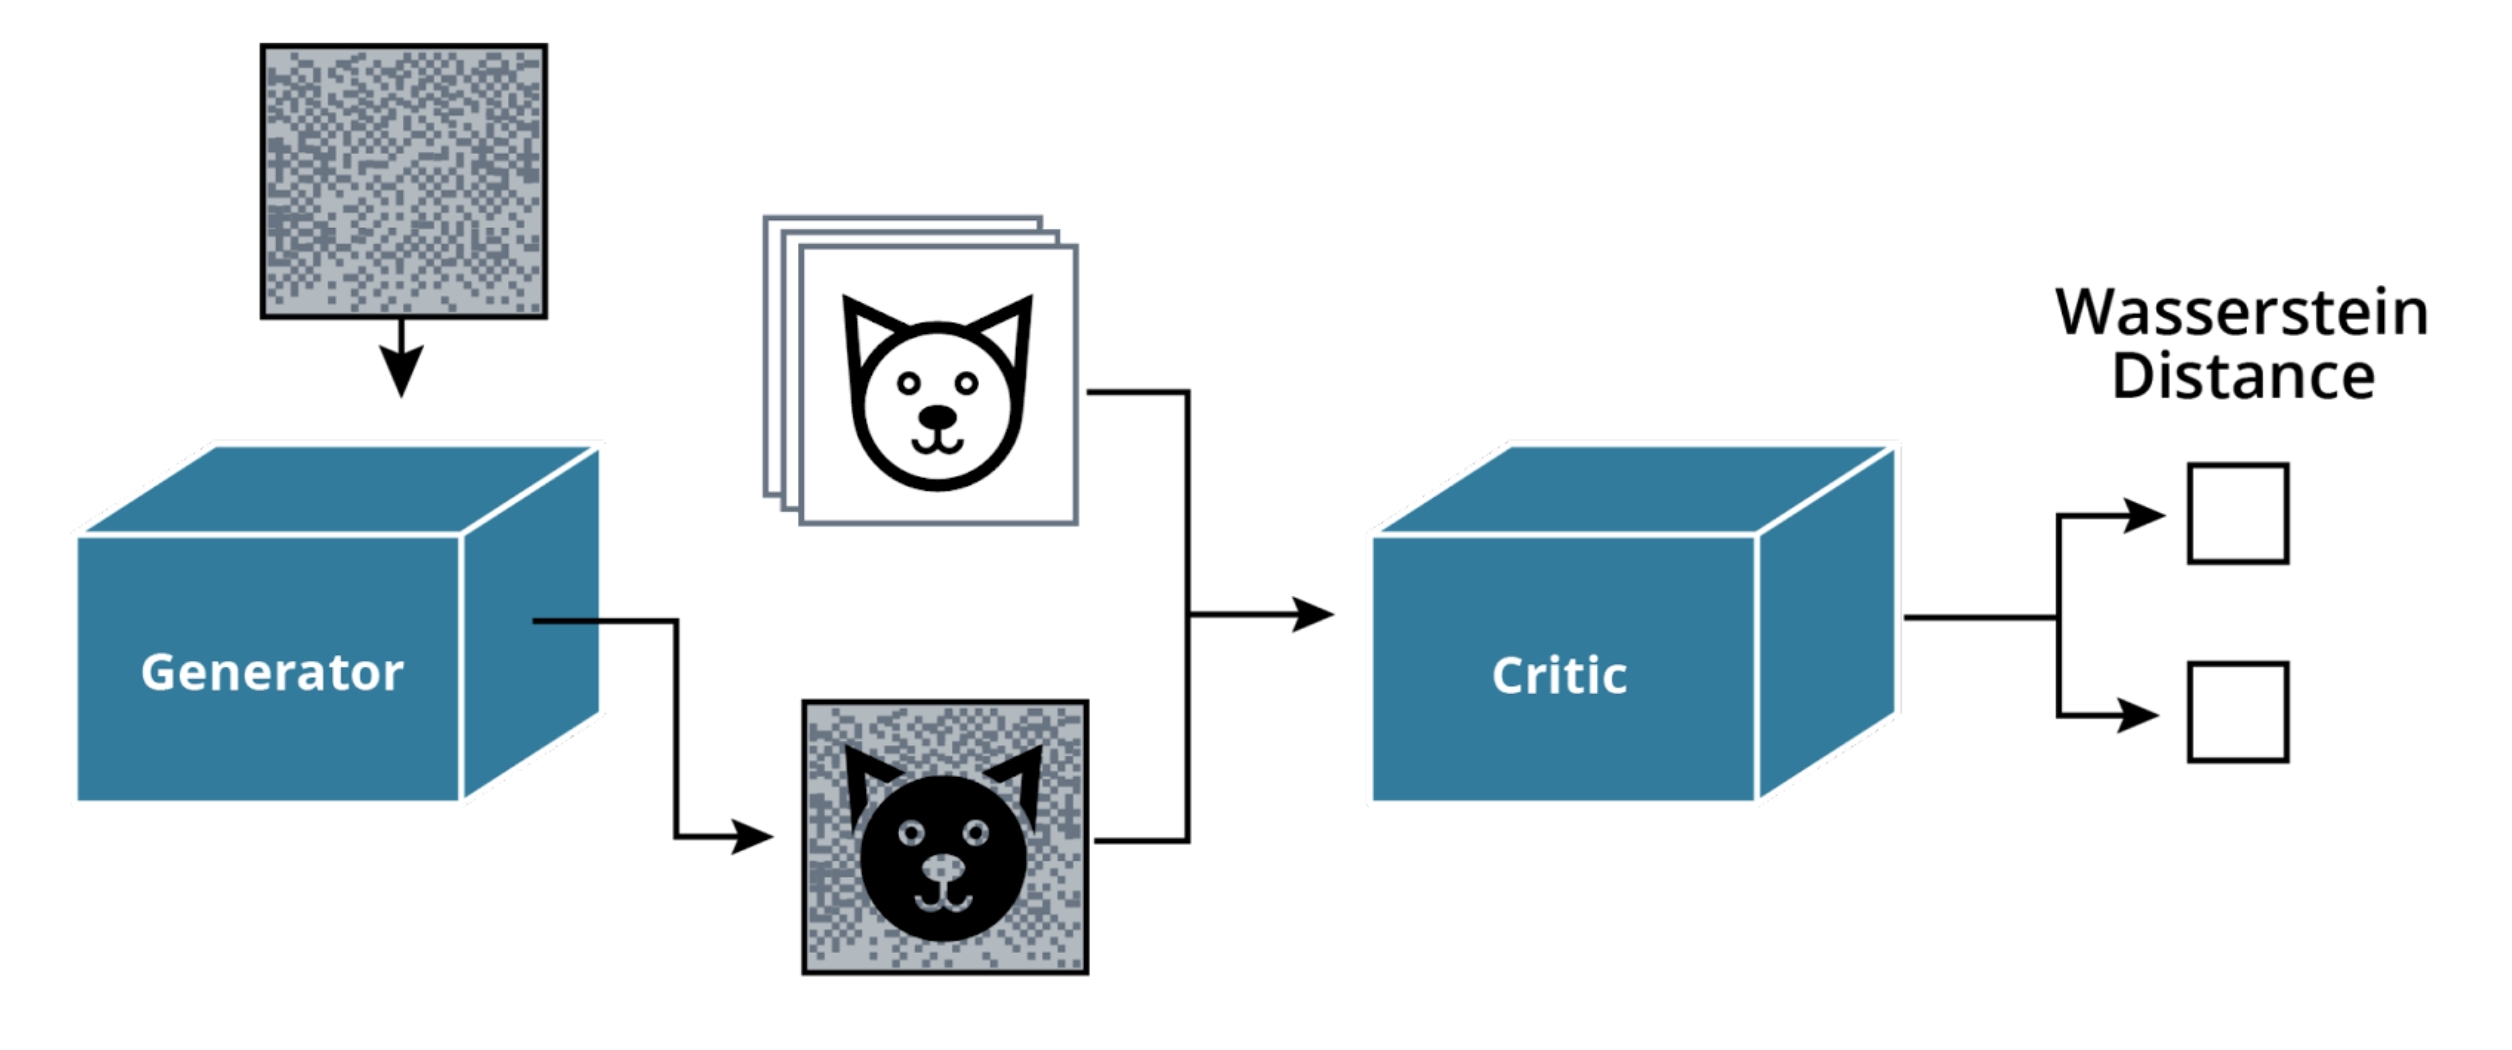
\includegraphics[width=0.75\linewidth]{img//genAdvNet//modernGAN/screen-shot-2022-05-12-at-12.06.29-pm.jpeg}
\captionof{figure}{Schematic representation of GAN architecture}

\section{Lesson Outline}
\href{https://www.youtube.com/watch?v=z4ylfVBgHW8&t=3s}{Youtube} \newline

In this lesson on \textbf{Modern GANs}, you will:

\begin{itemize}
    \item Use the Wasserstein Distance as a Loss Function for Training GANs
    \item Leverage Gradient Penalties to Stabilize GAN Model Training
    \item Build a ProGAN Model
    \item Build Components of a StyleGAN Model
\end{itemize}

\section{Limitations of the BCE Loss}
\href{https://www.youtube.com/watch?v=hlQQhQbRbTY&t=1s}{Youtube} \newline 
The original \href{https://arxiv.org/pdf/1406.2661.pdf}{\textbf{GAN paper}} [1] already mentions some of the limitations of the BCE Loss, in the section 6 \textit{'Advantages and disadvantages'}.

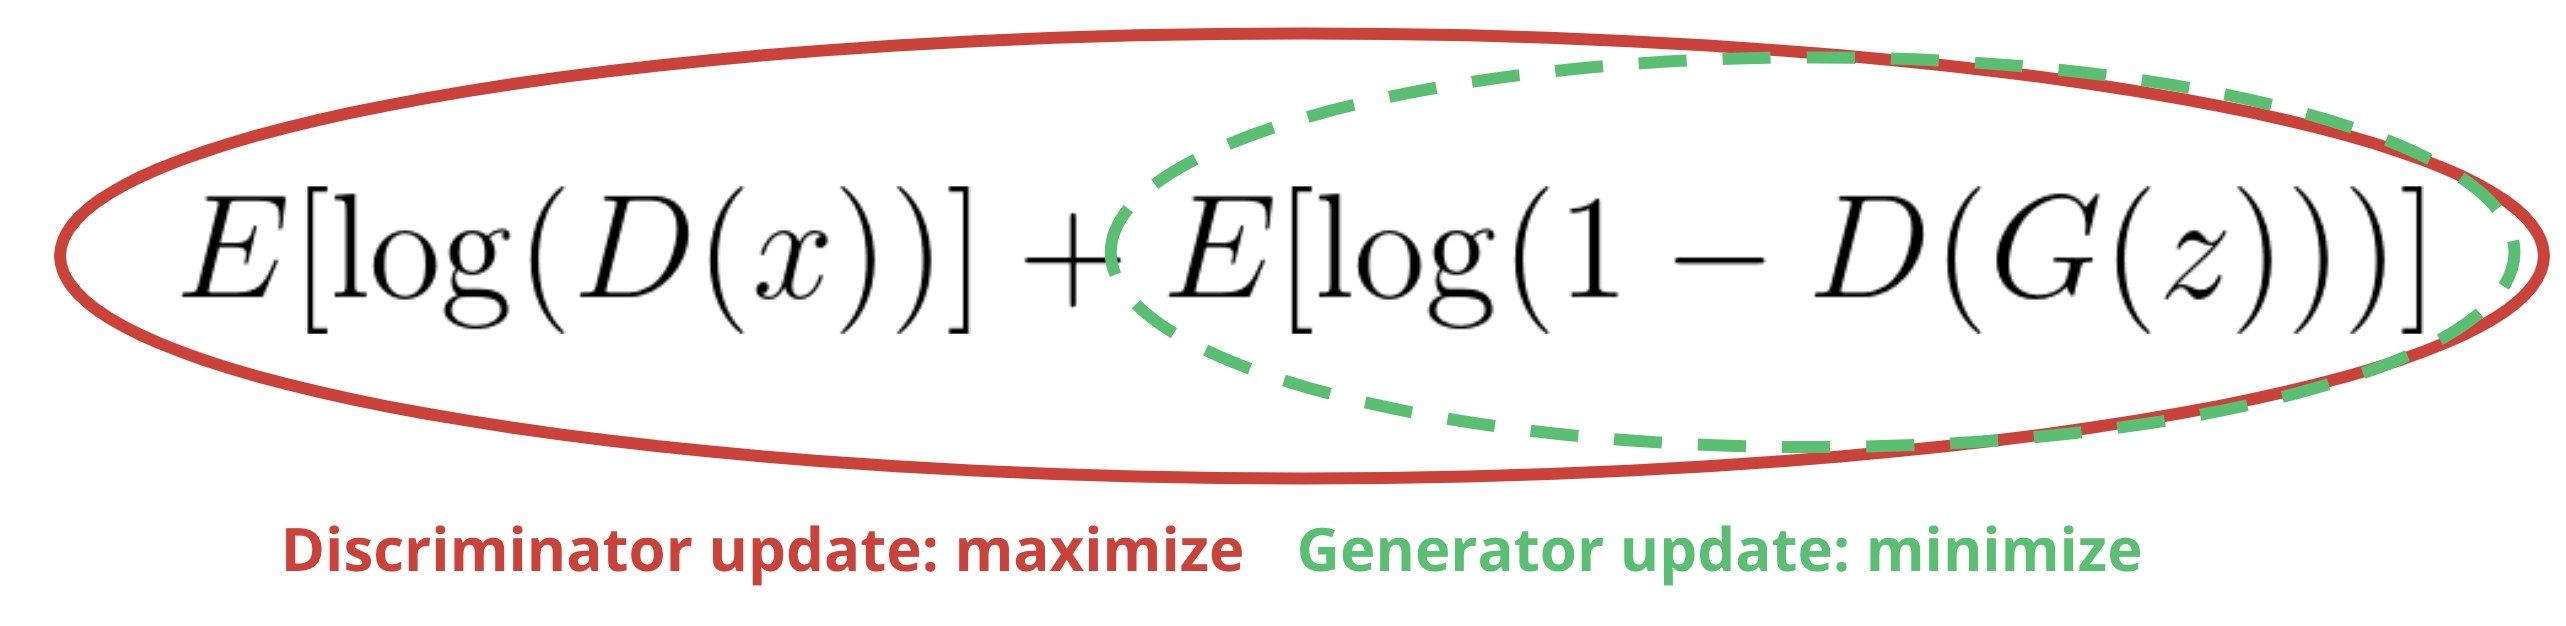
\includegraphics[width=1\linewidth]{img//genAdvNet//modernGAN/screen-shot-2022-06-29-at-4.13.01-pm.jpeg}
\captionof{figure}{The MiniMax game}

This is the minimax game that you should be familiar with. \[E[\log (D(x))] + E[\log (1 - D(G(z)))]\]

\begin{itemize}
    \item We have \(x\), a sample from our real distribution, \(z\) the latent vector, our discriminator \(D\), and our generator \(G\).
    \item The discriminator tries to maximize this expression, which means maximizing the log probability of \(x\) being real and maximizing the log of the inverse probability of \(G(z)\) being real.
    \item The generator tries to minimize the log of the inverse probability of \(G(z)\) being real.
    \item It is more stable for the generator to maximize the log probability of \(G(z)\) being fake.
\end{itemize}

\subsection{Challenges of Training GANs}
The common problems with GANs are:
\begin{itemize}
    \item \textbf{Mode Collapse} occurs when the generator only creates some of the modes of the real distribution. The generator is not penalized for focusing on a single mode with BCE loss. E.g. in case of the MNIST dataset: it would only produce 1 or 2 different digits
    \item \textbf{Vanishing Gradient} occurs when the discriminator loss reaches zero and the generator is not learning anymore.
\end{itemize}

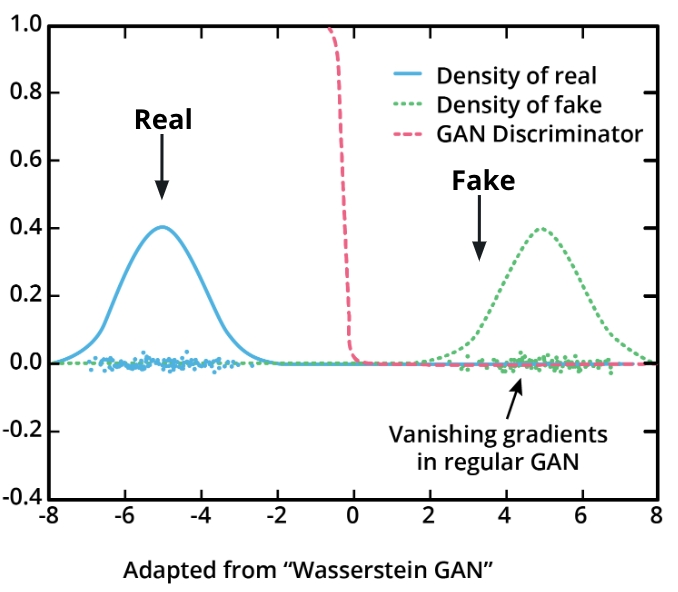
\includegraphics[width=0.5\linewidth]{img//genAdvNet//modernGAN/screen-shot-2022-06-29-at-4.23.02-pm.jpeg}
\captionof{figure}{Vanishing gradients in Generative Adversarial Networks (GANs)}


\subsection{Addressing Vanishing Gradients}
\textbf{Least squares} (LSGANs) can partly address the vanishing gradient problem for training deep GANs.
The problem is as follows:
\begin{itemize}
    \item \textbf{For negative log-likelihood loss}, when an input x is quite big, the gradient can get close to zero and become meaningless for training purposes. However, with a squared loss term, the gradient will actually increase with a larger x, as shown below.
\end{itemize}

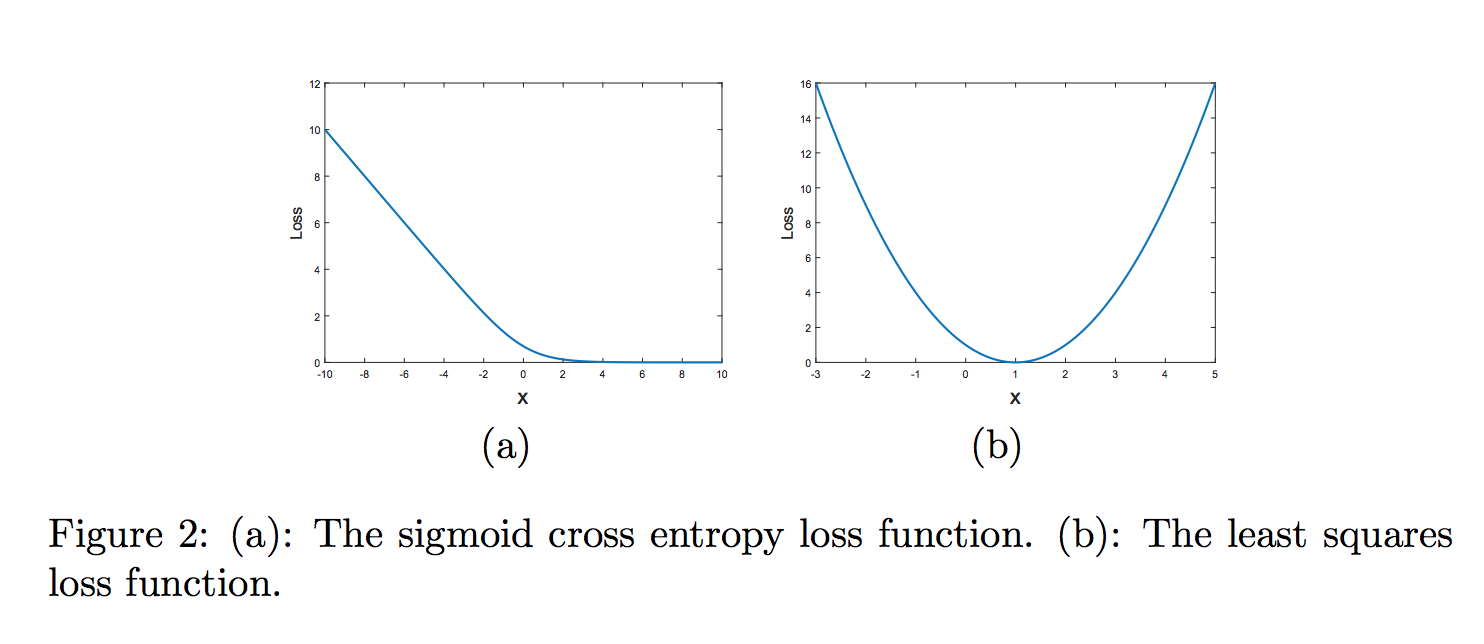
\includegraphics[width=0.75\linewidth]{img//genAdvNet//modernGAN/screen-shot-2018-11-10-at-7.38.03-pm.png}
\captionof{figure}{Loss patterns for large x\textit{x} values. Image from the \href{https://arxiv.org/abs/1611.04076}{\textbf{LSGAN paper}} [2].}

\textbf{Least square loss} is just one variant of a GAN loss. There are many more variants such as a \href{https://arxiv.org/abs/1701.07875}{\textbf{Wasserstein GAN loss}} [3] and others. \newline

These loss variants sometimes can help stabilize training and produce better results. As you write your own code, you're encouraged to hypothesize, try out different loss functions, and see which works best in your case!
\subsection{Citations}
Following are the full citations for the papers referenced on this page:

\begin{itemize}
    \item \textbf{[1]} I. Goodfellow, J. Pouget-Abadie, M. Mirza, et al, "\textit{Generative Adversarial Nets}", Departement d’informatique et de recherche operationnelle Universite de Montreal [Online], Available: \href{https://arxiv.org/pdf/1406.2661.pdf}{\textbf{https://arxiv.org/pdf/1406.2661.pdf}}. [Accessed June 28, 2022].
    \item \textbf{[2]} X. Mao, Q. Li, H. Xie, R. Y.K. Lau, et al, "\textit{Least Squares Generative Adversarial Networks}", Department of Computer Science, City University of Hong Kong, Department of Mathematics and Information Technology, The Education University of Hong Kong, et al [Online], Available: \href{https://arxiv.org/pdf/1611.04076.pdf}{\textbf{https://arxiv.org/pdf/1611.04076.pdf}}. [Accessed June 28, 2022].
    \item \textbf{[3]} M. Arjovsky, S. Chintala, and L. Bottou, "\textit{Wasserstein GAN}", Courant Institute of Mathematical Sciences, Facebook AI Research [Online], Available: \href{https://arxiv.org/pdf/1701.07875.pdf}{\textbf{https://arxiv.org/pdf/1701.07875.pdf}}. [Accessed June 28, 2022].
\end{itemize}

\section{Wasserstein Loss}
\href{https://www.youtube.com/watch?v=9LmWLMxNoF0}{Youtube} \newline

To prevent mode collapse and vanishing gradient (does not have zero gradient when when the real and fake distributions are very different) there is another loss function to train GANs: 
\begin{itemize}
    \item \textbf{The Earth Mover Distance or Wasserstein Metric} also referred to as \textbf{Wasserstein Loss} and \textbf{Wasserstein Distance}
\end{itemize}
This metric measures the distance between two distribution. The name Earth Mover's Distance comes from the following analogy: if each one of our distribution is a pile of dirt, the earth mover distance is the cost of turning one pile into another. 

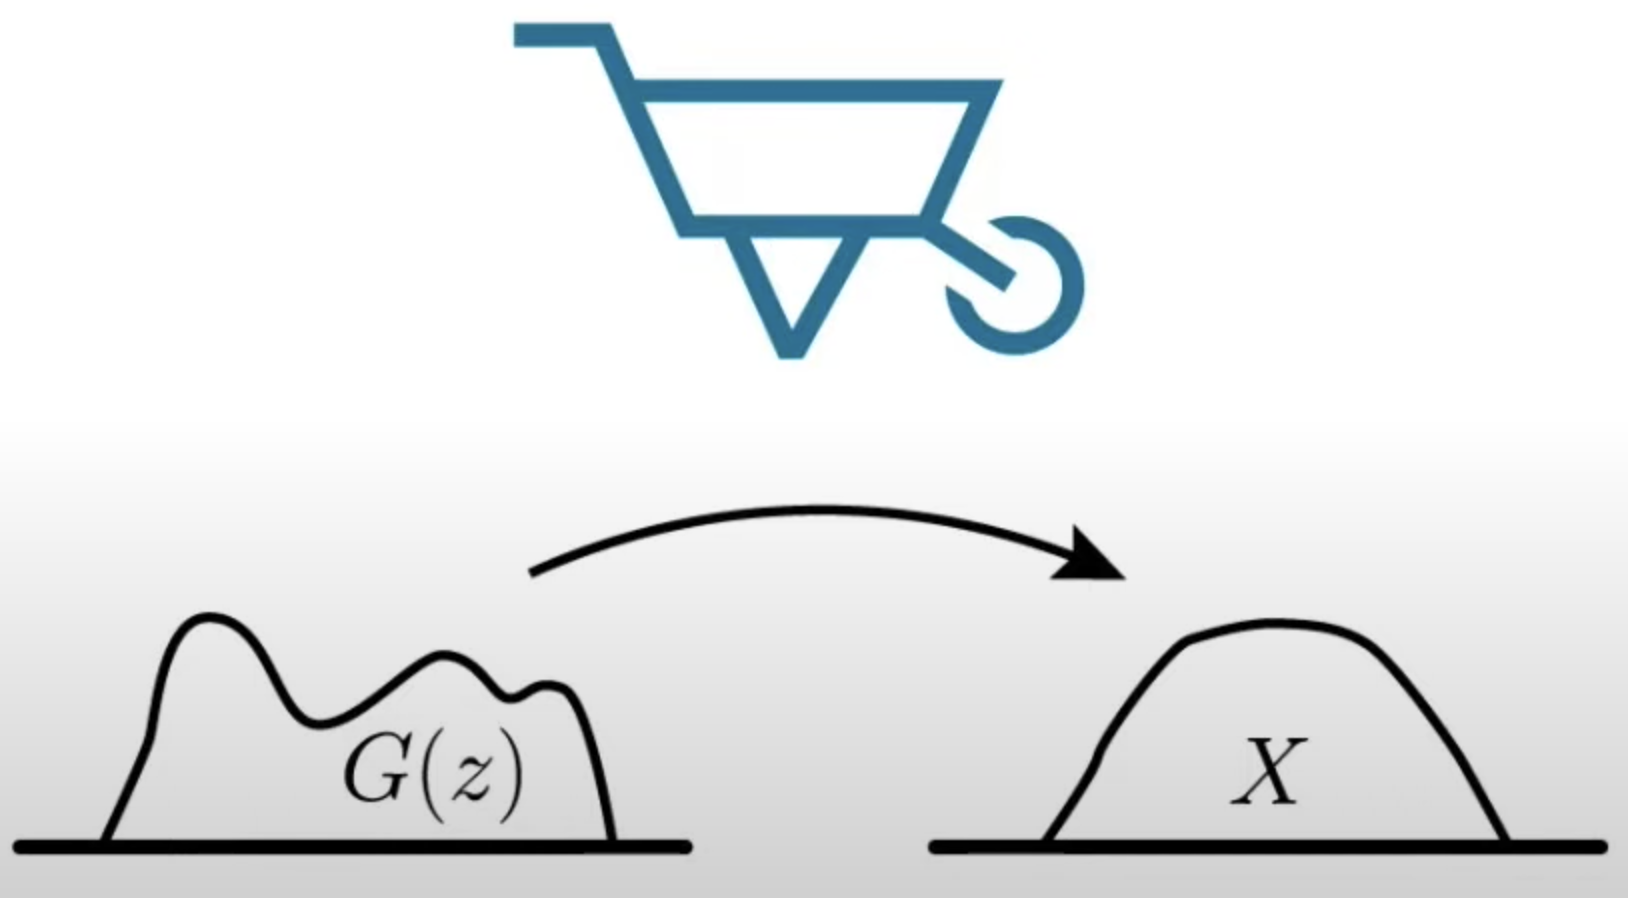
\includegraphics[width=0.5\linewidth]{img//genAdvNet//modernGAN/eathMoversDistance.png}

The Wasserstein Loss is mathematically represented as follows: \[E[C(x)] - E[C(G(z))]\]
Similar to the BCE Loss, note that the logs have disappeared. Indeed the Wasserstein distance gets rid of the log function and only considers the probabilities.

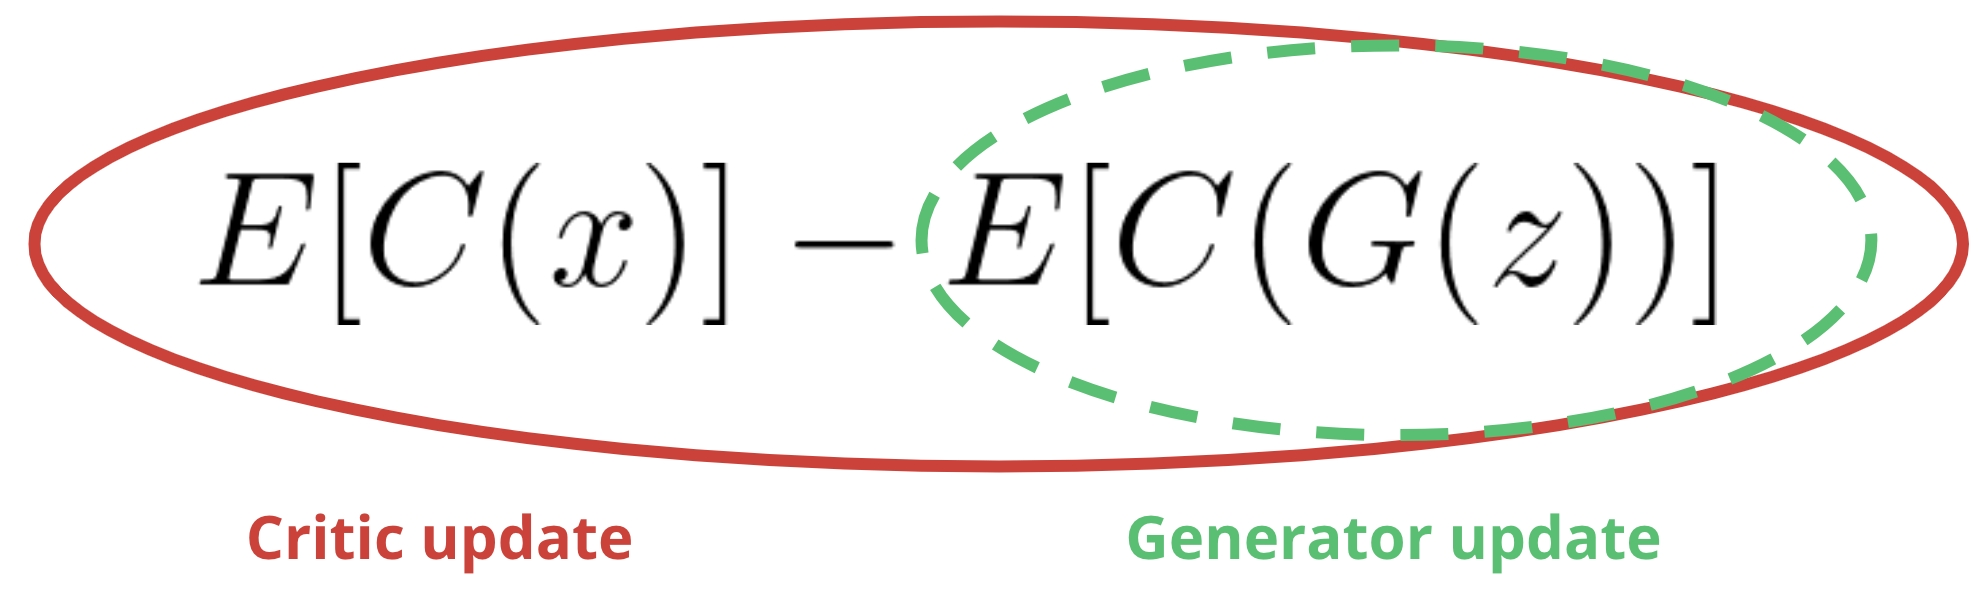
\includegraphics[width=0.5\linewidth]{img//genAdvNet//modernGAN/screen-shot-2022-06-29-at-4.29.11-pm.jpeg}
\captionof{figure}{The discriminator is now a critic!}

With the Wasserstein distance the discriminator is called \textbf{Critic}. \newline

The \textbf{Critic}:
\begin{itemize}
    \item Does not discriminate between real and fake anymore but instead measures the distance between both distributions.
    \item Will try to maximize this expression.
    \item Wants to maximize the score of the real distribution and minimize the score of the fake distribution, which is similar to maximizing its inverse.
\end{itemize}
The generator will try to maximize the critic score of the fake distribution, which is similar to minimizing it with the flipped label.

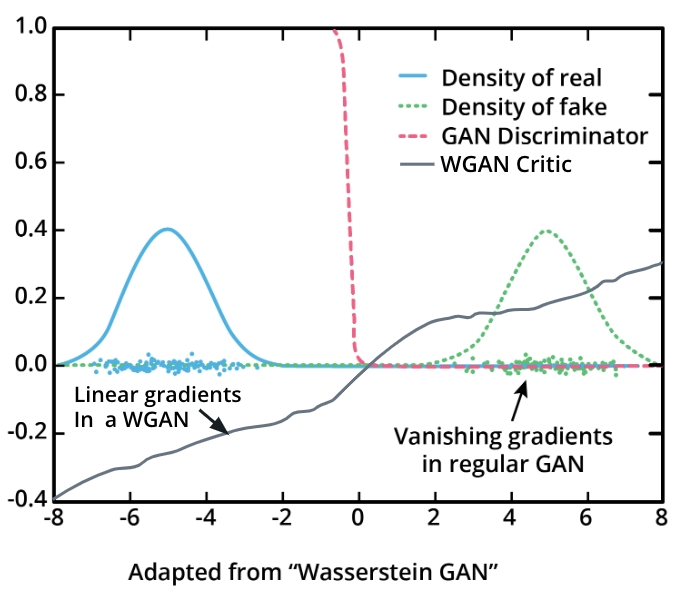
\includegraphics[width=0.75\linewidth]{img//genAdvNet//modernGAN/screen-shot-2022-06-29-at-4.33.14-pm.jpeg}
\captionof{figure}{\textbf{The Gradient of the Wasserstein Distance in Never Zero}}

The WGAN minimax game is described by the formula above. \newline

When training the critic \(C\), we want to maximize the critic score on the real images x and minimize the critic score on the fake images \(G(z)\) which is similar to maximizing the inverse of \(C(G(z))\). \newline

When training the generator \(G\), we want to maximize the score of the critic for the fake images.

\subsubsection{1-Lipschitz continuous}

The \textbf{1-Lipschitz continuous} is a new constraint on the discriminator or critic when using the Wasserstein distance as a loss function.\newline

Defined mathematically: \newline

For a function \(f\), the following condition must be fulfilled: \(|\frac{df(x)}{dx}| \le 1 \) \newline

\textbf{Note:} For the rest of the class, Critic and Discriminator will be used interchangeably to designate the Discriminator network.

\subsection{BCE Loss vs Wasserstein Loss}

\begin{table}[!htbp]
    \centering
    \begin{tabular}{c|c}
         Binary Cross Entropy & Wasserstein Distance\\
         \hline
         \(E[\log(D(x))] - E[\log(D(G(z)))]\)& \(E[C(x)] - E[C(G(z))])\)\\
         Discriminate between 0 and 1 & Critic outputs any real number\\
         Does not require any additional constraint & Requires 1-Lipschitz continuity on the critic\\
    \end{tabular}
\end{table}

\subsection{Additional Resources}

The \href{https://arxiv.org/pdf/1701.07875.pdf}{\textbf{Wasserstein GAN}} (WGAN) [1] paper is a little math-heavy but I recommend reading the paragraph on weight clipping on page 7 as well as the description of the WGAN algorithm on page 8.

\subsection{Quiz Question}
Which ones of the following are true about the BCE Loss?
\begin{itemize}
    \item \textbf{The output of the discriminator is bounded between 0 and 1}
    \item Requires the discriminator to be 1-Lipschitz continuous
    \item Can lead to vanishing gradients when the real and fake distributions are very similar.
    \item \textbf{Can lead to mode collapse.}
\end{itemize}

\subsection{Citations}
Following is the full citation for the paper referenced on this page:

\textbf{[1]} M. Arjovsky, S. Chintala, and L. Bottou, "\textit{Wasserstein GAN}", Courant Institute of Mathematical Sciences, Facebook AI Research [Online], Available: \href{https://arxiv.org/pdf/1701.07875.pdf}{\textbf{https://arxiv.org/pdf/1701.07875.pdf}}. [Accessed June 28, 2022].

\section{Gradient Penalties}
\href{https://www.youtube.com/watch?v=NqEUeISsqs8&t=5s}{Youtube} 
\subsection{Weight Clipping}
In the \href{https://arxiv.org/pdf/1701.07875.pdf}{\textbf{WGAN paper}} [1], the authors explain that:

\begin{quote}
\textit{Weight clipping is a} \textit{\textbf{clearly terrible way}} \textit{to enforce a Lipschitz constraint. If the clipping parameter is large, then it can take a long time for any weights to reach their limit, thereby making it harder to train the critic till optimality. If the clipping is small, this can easily lead to vanishing gradients when the number of layers is big, or batch normalization is not used (such as in RNNs). We experimented with simple variants (such as projecting the weights to a sphere) with little difference, and} \textit{\textbf{we stuck with weight clipping due to its simplicity and already good performance.}} \textit{However, we do leave the topic of enforcing Lipschitz constraints in a neural network setting for further investigation, and we actively encourage interested researchers to improve on this method.}

\end{quote}
\subsection{WGAN Training Algorithm}
To train the GAN:
\begin{itemize}
    \item Sample from the real data and generate some fake samples
    \item Then calculate the Wasserstein Distance and the gradients at line 5.
    \item Line 6, we perform backpropagation using RMSprop, an optimization algorithm similar to stochastic gradient descent or Adam
    \item Enforce the weights to stay within a threshold of -0.01 and 0.01
\end{itemize}
\begin{lstlisting}
# WGAN algorithm

1 while GAN has not converged:
2    # for each iteration
3    Sample a batch of real data
4    Sample a batch of fake data
5    Calculate the gradient gw
6    Backpropagation w = w + a RMSProp
7    w = clip(w, -c, c)
\end{lstlisting}
In short, weight clipping works, but is not the best approach to enforce the Lipschitz constraint.
\subsection{Gradient Penalties}
The WGAN-GP paper introduced the concept of \textbf{gradient penalty}. In this paper, the authors add a new term to the new loss function that will penalize high gradients and help enforce the 1-Lipschitz constraint. Added to the Wasserstein Loss formula was the gradient penalty:  \[\lambda E[(||\nabla_{\hat{x}} C(\hat{x})||_2- 1)^2]\]

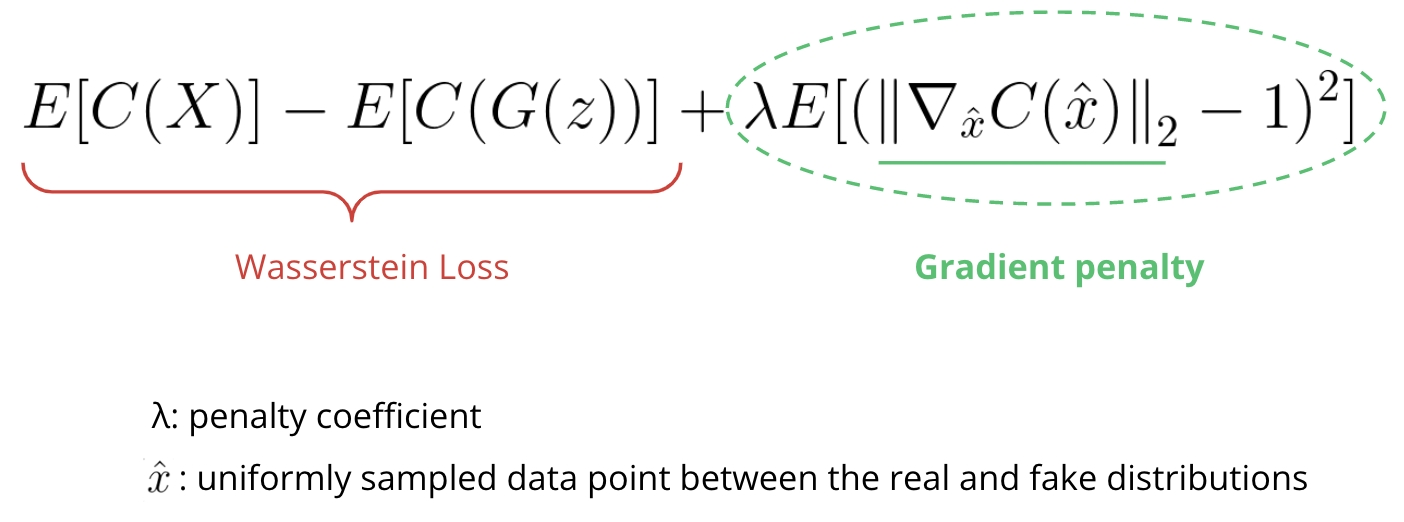
\includegraphics[width=1\linewidth]{img//genAdvNet//modernGAN/screen-shot-2022-06-29-at-4.56.30-pm.jpeg}
\captionof{figure}{Mathematical representation of gradient penalty}

Calculating the gradient penalty also includes a bit of interpolation of the real and fake distribution:
\begin{enumerate}
    \item Randomly sample a coefficient \(\alpha\) of between \(0\) and \(1\)
    \item Calculate the interpolation as: \(\hat{x} = \alpha x + (1 - \alpha) G(z)\)
\end{enumerate}
When \(\alpha\) is closer to \(0\) the interpolated sample is very noisy, and when \(\alpha\) is closer to \(1\) the interpolated sample is closer to the real distribution.
\subsection{Enforcing 1-Lipschity Continuity}
\begin{table}[!htbp]
    \centering
    \begin{tabular}{c|c}
         Weight clipping & Gradient Penalty\\
         \hline
         \(w \leftarrow clip(w, -c, c)\) & \(\lambda E[(||\nabla_{\hat{x}} C(\hat{x})||_2- 1)^2]\)\\
         Easy to implement, suboptimal way of enforcing the Lipschitz constraint & Requires calculating \(\hat{x}\), an interpolated ample of the real and fake distributions \(\alpha x + (1 - \alpha) G(z)\)\\
    \end{tabular}

\end{table}

\subsection{Additional Resources}
\begin{itemize}
    \item For additional discussion regarding weight clipping in PyTorch, check out \href{https://discuss.pytorch.org/t/how-to-do-constrained-optimization-in-pytorch/60122}{\textbf{How to do constrained optimization in PyTorch}}.
    \item A great GitHub repository,\href{https://github.com/LynnHo/DCGAN-LSGAN-WGAN-GP-DRAGAN-Pytorch}{\textbf{ DCGAN-LSGAN-WGAN-GP-DRAGAN-Pytorch}}, contains the implementation of various GANs with different gradient penalties. Reading the code is recommended as it will be helpful for the following exercises.
\end{itemize}

\subsection{Citations}
Following is the full citation for the paper referenced on this page: 
\begin{itemize}
    \item \textbf{[1]} M. Arjovsky, S. Chintala, and L. Bottou, "\textit{Wasserstein GAN}", Courant Institute of Mathematical Sciences, Facebook AI Research [Online], Available: \href{https://arxiv.org/pdf/1701.07875.pdf}{\textbf{https://arxiv.org/pdf/1701.07875.pdf}}. [Accessed June 28, 2022].
\end{itemize}

\section{Exercise 1: Wasserstein Loss and Gradient penalty}
In the course, we discussed the limitations of the binary cross entropy
loss (BCE Loss). It can lead to: 
\begin{itemize}
\item \href{https://developers.google.com/machine-learning/gan/problems}{mode collapse}: when the generator is stuck in a single mode of the distribution it is trying to replicate. For example, a generator training on the MNIST dataset would be stuck in generating images of certain digits only, as shown below.

    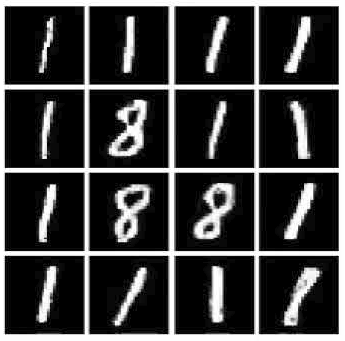
\includegraphics[width=0.5\linewidth]{img//genAdvNet//modernGAN/collapse.png}

\item vanishing gradient: it's a common problem with many neural networks architectures but is very common when training GANs. Because the discriminator's task is much easier than the generator's, the discriminator tends to converge faster and reach a high accuracy. The discriminator loss gets close to zero and the gradients become very small, leading to that vanishing gradient problem.
\end{itemize}

In this notebook, you will: 
\begin{itemize}
    \item implement the Wasserstein Loss
    \item implement two types of gradient penalties
\end{itemize}

\subsection{Wasserstein Loss}

The \href{https://arxiv.org/pdf/1701.07875.pdf}{Wasserstein GAN paper}
introduced a new type of loss function: the
\href{https://en.wikipedia.org/wiki/Wasserstein_metric}{Wasserstein
Distance}. We are now reshaping the problem GANs are solving: instead of
having a loss function that classifies a distribution as being real or
not, we have a loss function that tries to minimize the distance between
the real and the fake distribution. The difference is subtle but plays a
big role in the stability of GANs

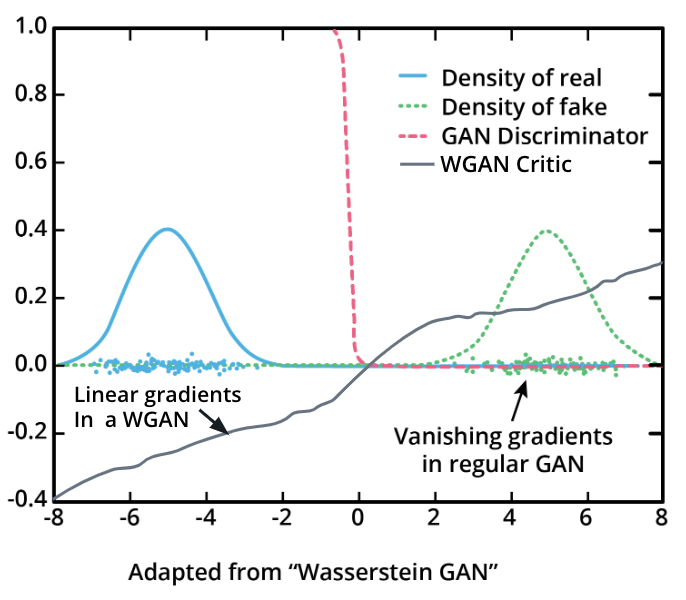
\includegraphics[width=0.75\linewidth]{img//genAdvNet//modernGAN/gradient_replace.png}

The discriminator is now called a \textbf{critic} because it's job is
not really to distinguish between real and fake anymore but to maximize
the distance between the two distributions. However, we will be using
both terms interchangeably for the sake of clarity. \newline

The Wasserstein loss can be calculated using the formula below:

\[\min_{g} \max_{c} E(c(x)) - E(c(g(z)))\]

You are now familiar with the minimax function. The main difference with
the BCE Loss is the disapperance of the logs!

\subsubsection{First exercise: implement the Wasserstein Loss}

The Wasserstein Loss (W-Loss) is taking the vector of logits outputed by
the discriminator as input. In comparison, the BCE Loss was taking the
probabilities (logits after a softmax layer) as inputs. The
discriminator W-Loss is trying to maximize the mean value of the logits
of real images and minize the mean value of the logits of fake images.
The generator W-Loss is trying to maximize the mean value of the logits
of fake images.

\begin{lstlisting}[language=Python]
import torch

import tests
\end{lstlisting}

\begin{lstlisting}[language=Python]
def disc_w_loss(real_logits: torch.Tensor, fake_logits: torch.Tensor):
    """
    Wasserstein Discriminator Loss
    
    args:
    - real_logits: vector of logits outputed by the discriminator with a real input image
    - fake_logits: vector of logits outputed by the discriminator with a fake input image 
    """
    real_loss = -real_logits.mean()
    fake_loss = fake_logits.mean()
    return real_loss + fake_loss
\end{lstlisting}

\begin{lstlisting}[language=Python]
def disc_g_loss(fake_logits: torch.Tensor):
    """
    Wasserstein Generator Loss
    
    args:
    - fake_logits: vector of logits outputed by the discriminator with a fake input image 
    """
    fake_loss = -fake_logits.mean()
    return fake_loss
\end{lstlisting}

\begin{lstlisting}[language=Python]
tests.check_disc_w_loss(disc_w_loss)
\end{lstlisting}

\begin{lstlisting}[language=Python]
tests.check_gen_w_loss(disc_g_loss)
\end{lstlisting}

\subsection{Gradient penalty}

To train a GAN with the Wasserstein Loss, the discriminator (or critic)
must be
\href{https://en.wikipedia.org/wiki/Lipschitz_continuity}{1-Lipschitz
continuous}. \newline

The 1-Lipschitz continuity constraint implies that the norm of the
gradient of the function must be below 1. In other words, for a function
\(f(x)\):

\[|| \frac{df}{dx} || < 1\]

Because the W-Loss is not bounded between 0 and 1 like the BCE loss, the
above constraint makes sure that the loss does not grow too much. \newline

In the original paper, the authors enforced this condition by using
weight clipping. However, per their own words:

\begin{lstlisting}
Weight clipping is a clearly terrible way to enforce a Lipschitz constraint. If the
clipping parameter is large, then it can take a long time for any weights to reach
their limit, thereby making it harder to train the critic till optimality. If the clipping
is small, this can easily lead to vanishing gradients when the number of layers is
big, or batch normalization is not used (such as in RNNs). We experimented with
simple variants (such as projecting the weights to a sphere) with little difference, and
we stuck with weight clipping due to its simplicity and already good performance.
However, we do leave the topic of enforcing Lipschitz constraints in a neural network
setting for further investigation, and we actively encourage interested researchers
to improve on this method.
\end{lstlisting}

\subsection{WGAN-GP}

Introducing Wasserstein Gan with Gradient Penalty, or
\href{https://arxiv.org/pdf/1704.00028.pdf}{WGAN-GP}. In this paper, the
author introduce a more robust way to enforce the 1-Lipschitz constaint
of the critic: a \textbf{gradient penalty term} in the loss function.
The new loss function is described below:

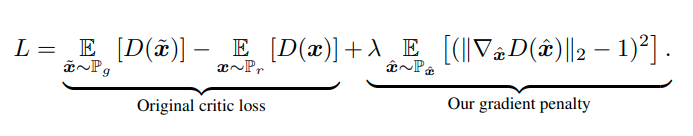
\includegraphics[width=1\linewidth]{img//genAdvNet//modernGAN/wgan_gp.png}

The gradient penalty is calculated as follow: 
\begin{itemize}
    \item sample a random point \(\hat{x}\) between the generated distribution and the real distribution.
    \item run this sample through the discriminator and calculate the gradient \(\nabla_{\hat{x}} D(\hat{x})\)
    \item calculate the L2 norm of the gradient \(|| \nabla_{\hat{x}} D(\hat{x}) ||_{2}\)
    \item remove 1, square the result and calculate the mean \((|| \nabla_{\hat{x}} D(\hat{x}) ||_{2} - 1) ^{2}\)
\end{itemize}

\subsubsection{Second exercise: implement the gradient penalty}
In the second exercise of this notebook, you will implement the above
gradient penalty. To help you, I have created a dummy critic module. \newline

\textbf{Tips}: 
\begin{itemize}
    \item to calculate the gradients, you first have to set the attribute of a tensor \lstinline{requires_grad} to True.
    \item you can use the following code to calculate the gradients:
\end{itemize}

\begin{lstlisting}
torch.autograd.grad(critic(x), x, grad_outputs=torch.ones_like(critic(x)), create_graph=True)[0]
\end{lstlisting}

\begin{lstlisting}[language=Python]
import torch.nn as nn
\end{lstlisting}

\begin{lstlisting}[language=Python]
class Critic(nn.Module):
    """ 
    Dummy critic class 
    """
    def __init__(self):
        super(Critic, self).__init__()
        
    def forward(self, x: torch.Tensor) -> torch.Tensor:
        return torch.pow(x, 2)
\end{lstlisting}

\begin{lstlisting}[language=Python]
def gradient_penalty(real_sample: torch.Tensor, 
                     fake_sample: torch.Tensor,
                     critic: nn.Module) -> torch.Tensor:
    """
    Gradient penalty of the WGAN-GP model
    args:
    - real_sample: sample from the real dataset
    - fake_sample: generated sample
    
    returns:
    - gradient penalty
    """
    # sample a random point between both distributions
    alpha = torch.rand(real_sample.shape)
    x_hat = alpha * real_sample + (1 - alpha) * fake_sample
    
    # calculate the gradient
    x_hat.requires_grad = True
    pred = critic(x_hat)
    grad = torch.autograd.grad(pred, 
                               x_hat, 
                               grad_outputs=torch.ones_like(pred), 
                               create_graph=True)[0]
    
    # calculate the norm and the final penalty
    norm = torch.norm(grad.view(-1), 2)
    gp = ((norm - 1)**2).mean()    
    return gp
\end{lstlisting}

\begin{lstlisting}[language=Python]
real_sample = torch.randn(3, 32, 32)
fake_sample = torch.randn(3, 32, 32)
critic = Critic()

gradient_penalty = gradient_penalty(real_sample, fake_sample, critic)
\end{lstlisting}

\subsection{DRAGAN}

The \href{https://arxiv.org/pdf/1705.07215.pdf}{DRAGAN paper} offered a
different approach to calculate the gradient penalty and enforce the
1-Lipschitz constraint on the critic.

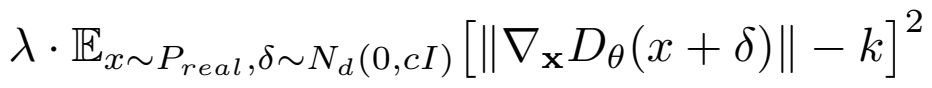
\includegraphics[width=1\linewidth]{img//genAdvNet//modernGAN/dragan_gp.png}
    
As you can see, the formula is very similar, especially since the
authors use \(k = 1\) for their experiments. The main difference with
the WGAN-GP gradient penalty is the \(\delta\) term, which is a noise
term. In their implementation, the authors calculate \(X_p = X + \delta\) as follow:

\[X_{p} = X + 0.5 * \sigma({X}) * N\]

where \(\sigma\) is the standard deviation and \(N\) a noise term
sampled from the uniform distribution. \newline

The gradient penalty is then calculated as follow: 
\begin{itemize}
    \item sample a random point \(\hat{x}\) between the real distribution \(X\) and \(X_{p}\) .
    \item run this sample through the discriminator and calculate the gradient \(\nabla_{\hat{x}} D(\hat{x})\)
    \item calculate the L2 norm of the gradient \(|| \nabla_{\hat{x}} D(\hat{x}) ||_{2}\)
    \item remove 1, square the result and calculate the mean \((|| \nabla_{\hat{x}} D(\hat{x}) ||_{2} - 1) ^{2}\)
\end{itemize}

\subsubsection{BCE Loss}
Interestingly, using this gradient penalty lifts some of the constraint
on the BCE Loss and the author use the above gradient penalty with the
vanilla GAN losses (BCE Loss).

\subsubsection{Third exercise: implement the DRAGAN gradient penalty}

In the third exercise of this notebook, you will implement the DRAGAN
gradient penalty. This is a one liner difference with the above
implementation!

\begin{lstlisting}[language=Python]
def gradient_penalty_dragan(real_sample: torch.Tensor, critic: nn.Module) -> torch.Tensor:
    """
    Gradient penalty of the WGAN-GP model
    args:
    - real_sample: sample from the real dataset
    
    returns:
    - gradient penalty
    """
    # sample a random point between both distributions
    X_p = real_sample + 0.5 * real_sample.std() * torch.rand_like(real_sample)
    
    alpha = torch.rand(real_sample.shape)
    x_hat = alpha * real_sample + (1 - alpha) * X_p
    
    # calculate the gradient
    x_hat.requires_grad = True
    pred = critic(x_hat)
    grad = torch.autograd.grad(pred, 
                               x_hat, 
                               grad_outputs=torch.ones_like(pred), 
                               create_graph=True)[0]
    
    # calculate the norm and the final penalty
    norm = torch.norm(grad.view(-1), 2)
    gp = ((norm - 1)**2).mean()
    return gp
\end{lstlisting}

\begin{lstlisting}[language=Python]
dragan_gp = gradient_penalty_dragan(real_sample, critic)
\end{lstlisting}

\section{WARNING}

The gradient penalty terms penalize each input to the critic
individually. Therefore, the critic should a single input to a single
output. However, we use some layers in the discriminator that remove
this property: the BatchNormalization layers. The authors of the WGAN-GP
paper explain the following:

\begin{quote}
No critic batch normalization Most prior GAN implementations use batch normalization in both the generator and the discriminator to help stabilize training, but batch normalization
changes the form of the discriminator’s problem from mapping a single input to a single output to
mapping from an entire batch of inputs to a batch of outputs . Our penalized training objective
is no longer valid in this setting, since we penalize the norm of the critic’s gradient with respect
to each input independently, and not the entire batch. To resolve this, we simply omit batch normalization in the critic in our models, finding that they perform well without it. Our method works
with normalization schemes which don’t introduce correlations between examples. In particular, we
recommend layer normalization as a drop-in replacement for batch normalization.
\end{quote}

Keep this in mind if you decide to use the gradient penalty in your
project!


\section{Exercise 1: Solution}
\href{https://www.youtube.com/watch?v=XcwpaN_qMLE}{Youtube}

\section{Progressive Growing of GANS}
\href{https://www.youtube.com/watch?v=jnVQRG0ocjk}{Youtube} \newline

To make training even more stable, the \textbf{ProGAN} model was developed and the current resolution is 16x16.
\subsection{How ProGAN works}
\begin{itemize}
    \item It adds a new layer to the generator and a new layer to the discriminator by fading the layers in smoothly.
    \item In the generator, the resolution of the 16x16 layer is doubled using an interpolation method such as nearest neighbor. The output of the 32x32 layer is then fused with this interpolated output.
    \item In the discriminator, the output of the 32x32 layer is fused with a downsampled image.
    \item A pooling method such as average pooling is used for downsampling.
\end{itemize}

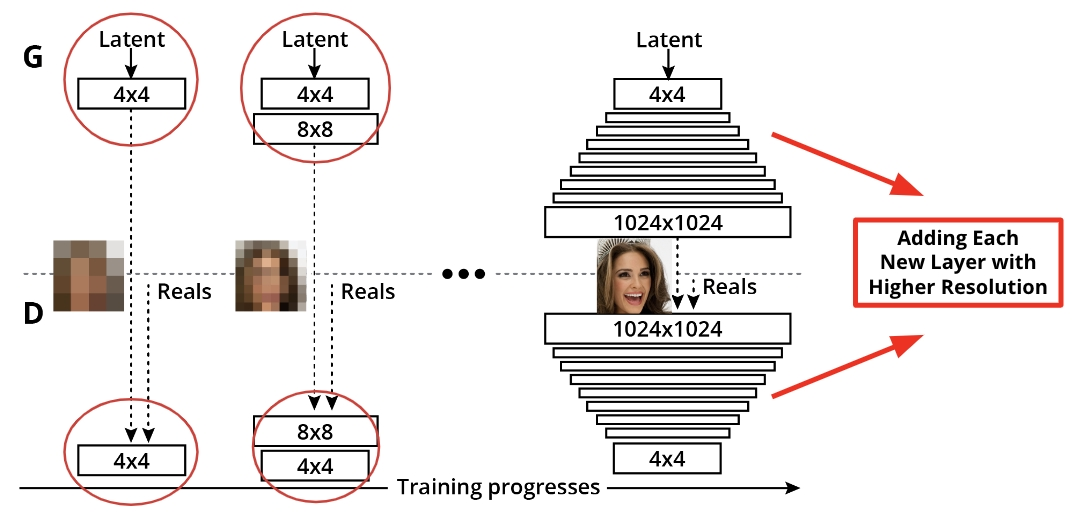
\includegraphics[width=1\linewidth]{img//genAdvNet//modernGAN/screen-shot-2022-06-30-at-1.47.23-pm.jpeg}
\captionof{figure}{ProGAN progressively adds layers at higher resolutions}

In both cases, perform a weighted sum of the learned output of the new layer with the non-parametric output of the previous layer. \newline

Slowly increase the weight of the output of the new layer over 10 epochs to reach a stage where there is no need to fade that layer anymore. \newline

Then train the network at the 32x32 resolution for another 10 epochs.
\subsection{Layer Fading}
For more stable training, \textbf{layer fading} is a way to incorporate new layers. Consider the following example:

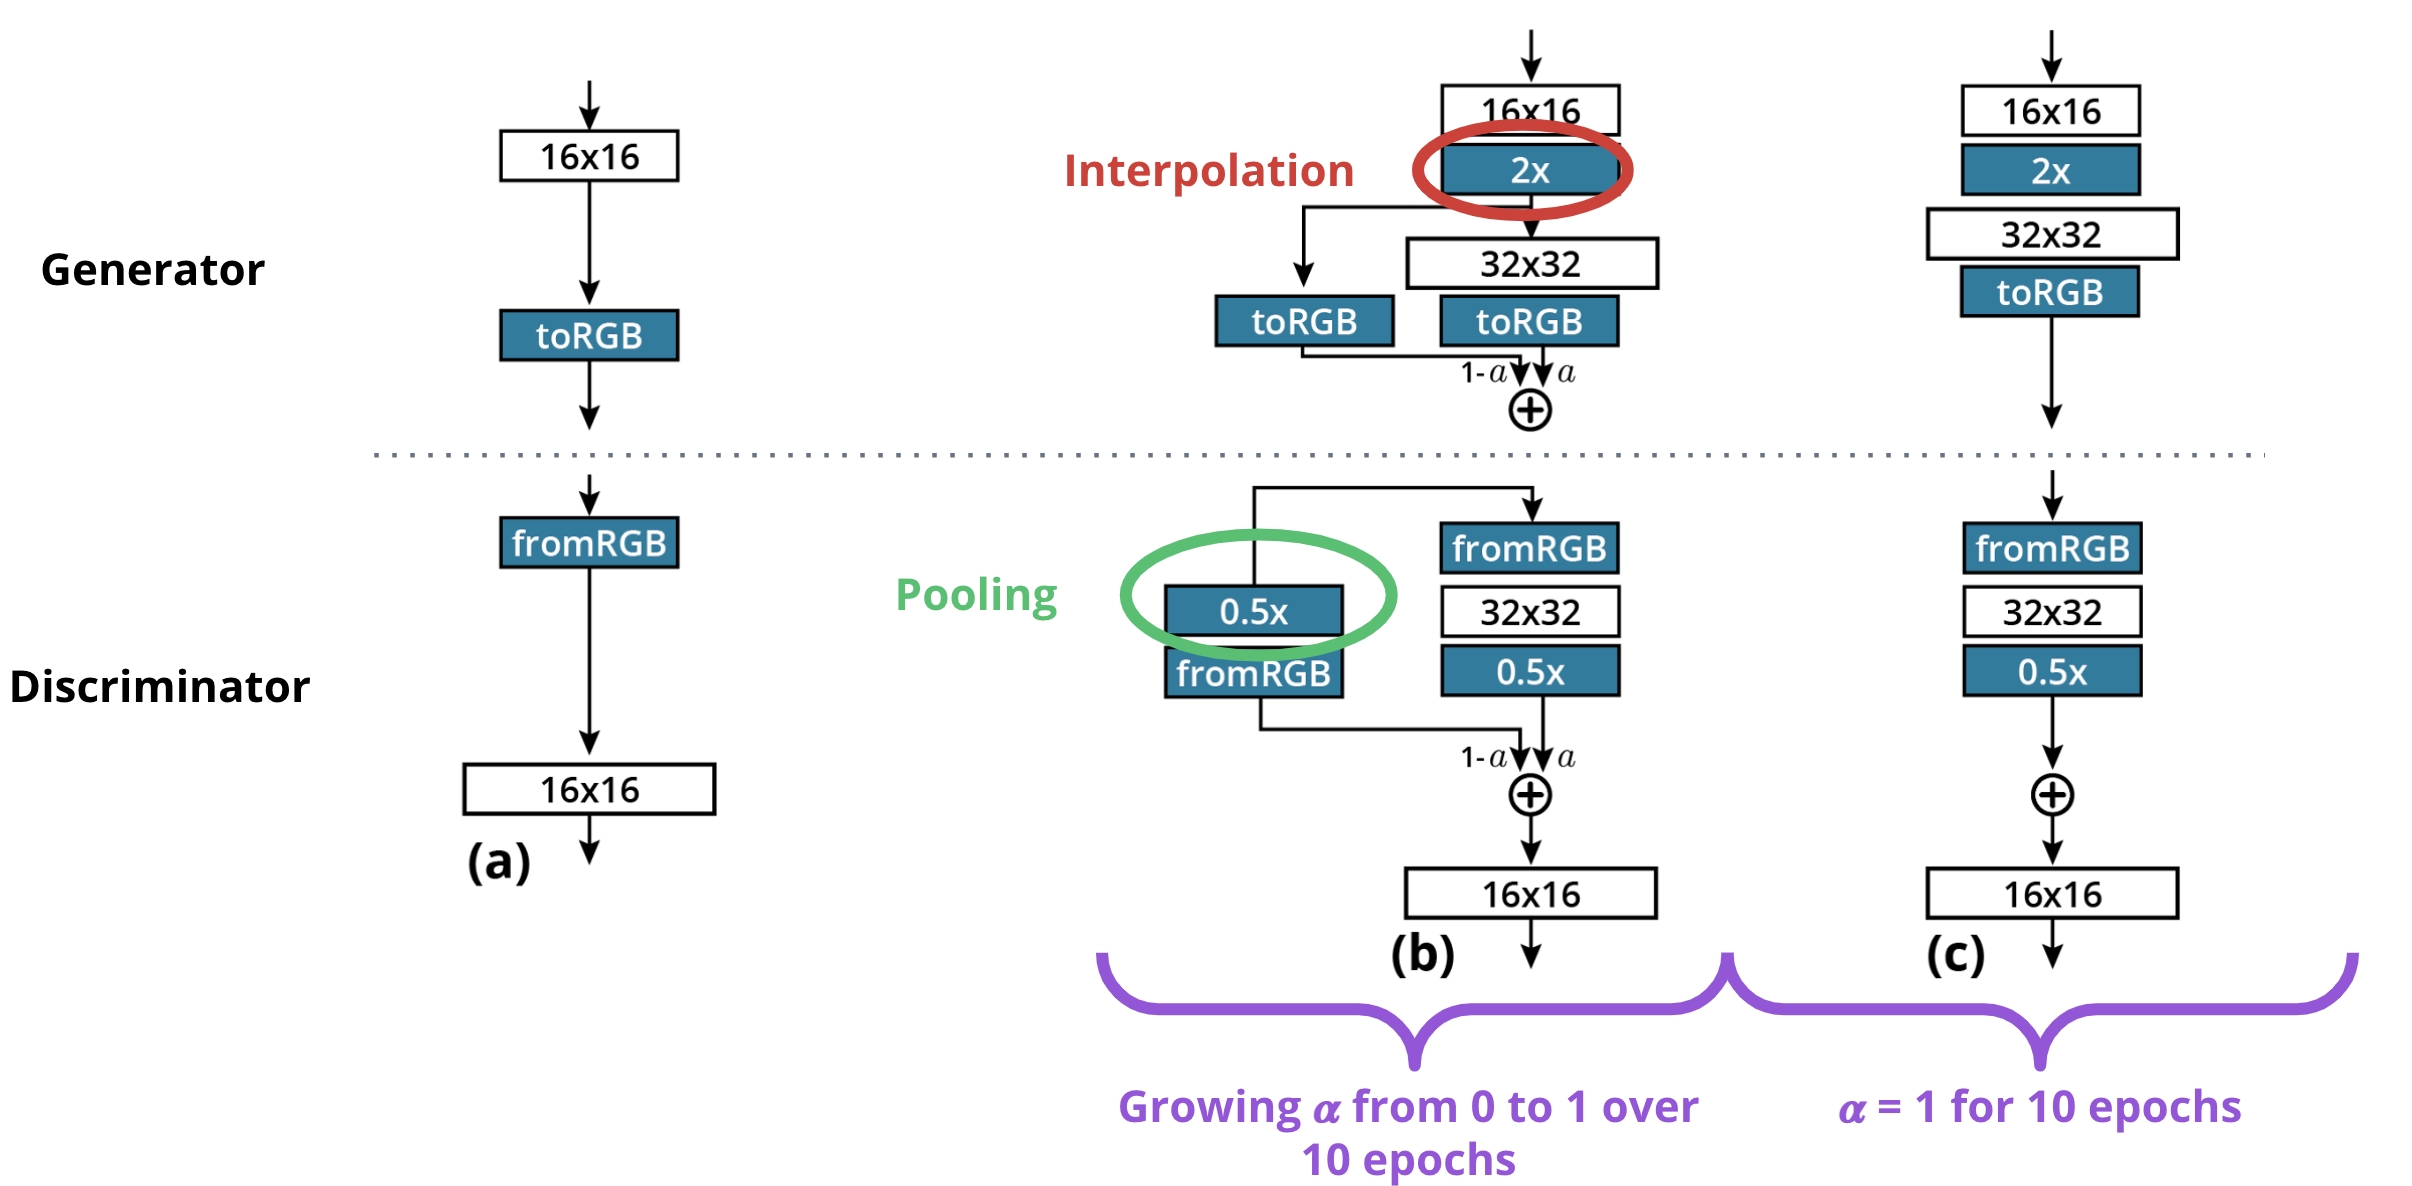
\includegraphics[width=1\linewidth]{img//genAdvNet//modernGAN/screen-shot-2022-06-30-at-1.50.56-pm.jpeg}
\captionof{figure}{Layer fading}


\begin{enumerate}
    \item Training a ProGAN model and the current resolution is 16x16. The toRGB layer maps the output of the last convolution to an RGB image and the from RGB layer takes a RGB image as input and feeds it into the next convolution layer.
    \item To increase the resolution to 32x32 use \textbf{layer fading}. Add a new layer to the generator and the discriminator by doubling the resolution of the 16x16 layer using an \textbf{interpolation} method such as nearest neighbor.
    \begin{itemize}
        \item In the generator, fuse the output of the 32x32 layer with the interpolated output.
        \item In the discriminator, fuse the output of the 32x32 layer with a downsampled image and use a pooling method such as average pooling for downsampling.
    \end{itemize}
    \item For both cases, perform a weighted sum of the learned output of the new layer with the non parametric output of the previous layer. Slowly increase the weight of the output of the new layer over 10 epochs to reach a stage where a fade is not needed in that layer.
    \item Train the network at the 32x32 resolution for another 10 epochs
\end{enumerate}

\subsection{ProGAN Tricks}

\begin{itemize}
    \item \textbf{Progressive Growing} – Progressively train layers and increase resolution
    \item \textbf{Minibatch Discrimination} – Enforce fake and real batches to have similar statistics
    \item \textbf{Equalized Learning Rates} – Scale the weights of each layer by a different constant to make sure the layers are learning at the same speed
    \item \textbf{Pixelwise Normalization} – Normalize each pixel of a feature map along the channel axis
\end{itemize}

\subsection{Additional Resources}

The ProGAN paper, \href{https://arxiv.org/pdf/1710.10196.pdf}{\textbf{Progressive Growing GANs for Improved Quality, Stability, and Variation}} [1], is very accessible and I recommend reading it to better understand the different components of ProGAN.

Other resources for implementing ProGAN include the following links:

\begin{itemize}
    \item \href{https://github.com/tkarras/progressive_growing_of_gans}{\textbf{Official ProGAN implementation in TensorFlow}}
    \item \href{https://github.com/akanimax/pro_gan_pytorch}{\textbf{\textbf{ProGAN implementation in PyTorch (unofficial)}
}}
\end{itemize}
\subsection{Quiz Question}
You are starting to train a ProGAN model. Put the following steps in the right order!

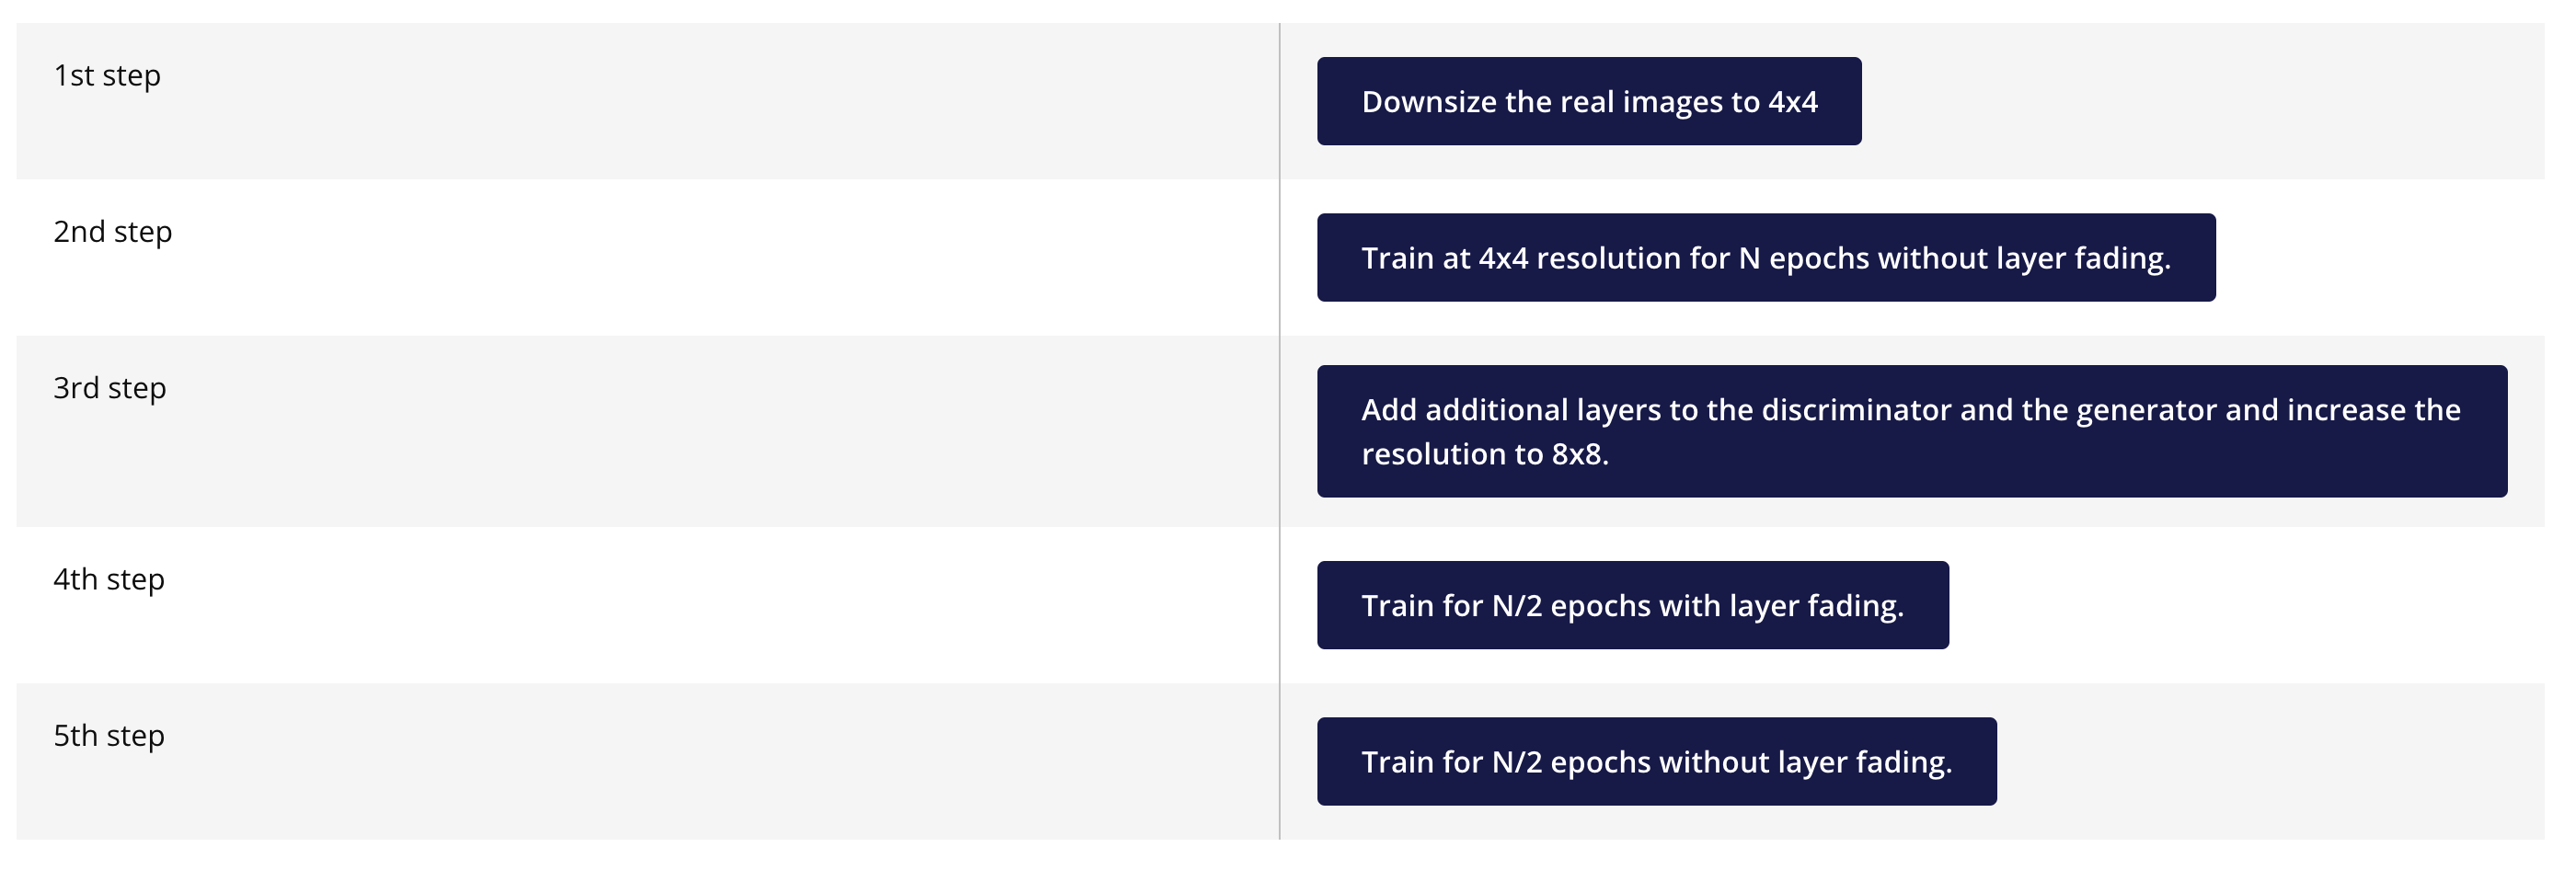
\includegraphics[width=1\linewidth]{img//genAdvNet//modernGAN/quizPGAN.png}

\subsection{Citations}

Following is the full citation for the paper referenced on this page: \newline

\textbf{[1]} I. T. Karras, T. Aila, S. Laine, J. Lehtinen, "\textit{Progressive Growing GANs for Improved Quality, Stability, and Variation}", NVIDIA, Aalto University [Online], Available: \href{https://arxiv.org/pdf/1710.10196.pdf}{\textbf{https://arxiv.org/pdf/1710.10196.pdf}}. [Accessed June 28, 2022].

\section{ProGAN components}
In addition to the progressive growing of networks, the \href{https://arxiv.org/pdf/1710.10196.pdf}{\textbf{ProGAN paper}} [1] has a couple of additional novel ideas: \textbf{pixelwise normalization} and \textbf{minibatch standard deviation}.

\subsection{Pixelwise normalization}

You are familiar with batch normalization and you may be familiar with other type of normalization, as described in the figure below.

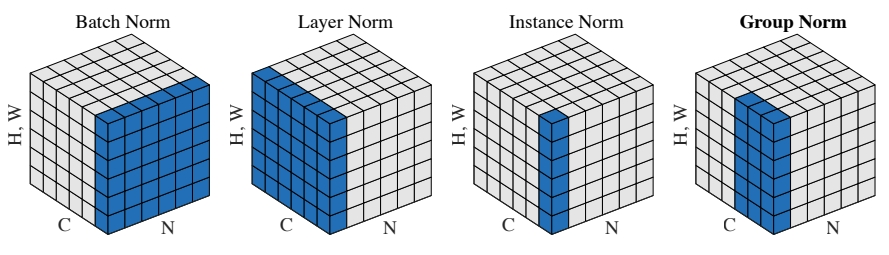
\includegraphics[width=1\linewidth]{img//genAdvNet//modernGAN/screenshot-from-2022-05-04-09-22-26.jpeg}
\captionof{figure}{From the paper, \href{https://arxiv.org/pdf/1803.08494.pdf}{\textbf{Group Normalization}}, by Yuxin Wu, et al [2]}

C is the channel dimensions, N the batch dimension and H, W the spatial dimensions. For example, for a batch normalization layer, we calculate mean and variance over the batch and spatial dimensions, so we have a pair of (mean, variance) values for each channel. \newline

With pixel normalization, we normalize each pixel of the input volume as follow:
\begin{lstlisting}
y = x.pow(2.0).mean(dim=1, keepdim=True).add(alpha).sqrt() 
x = x / y
\end{lstlisting}
where \lstinline|x| is the input volume of dimensions (NCHW). We square the input volume, calculate the mean over the channel dimension, add a very small factor alpha and calculate the square root.

\subsection{Minibatch Standard Deviation}
The paper, \href{https://arxiv.org/pdf/1606.03498.pdf}{\textbf{Improved Techniques for Training GANs}} [3], introduced the concept of \textbf{minibatch discrimination}, to enforce similarities between batches of real and fake images. \newline

In the ProGAN paper, the authors simplify this idea by introducing \textbf{minibatch standard deviation}. They create a new layer that adds a feature map to the input. This layer does the following:
\begin{itemize}
    \item calculate the standard deviation for each feature and spatials locations
    \item replicate the value and concatenate it over all spatial locations
\end{itemize}

\begin{lstlisting}
    def minibatch_stddev_layer(x, group_size=4):
    with tf.variable_scope('MinibatchStddev'):
        group_size = tf.minimum(group_size, tf.shape(x)[0])     # Minibatch must be divisible by (or smaller than) group_size.
        s = x.shape                                             # [NCHW]  Input shape.
        y = tf.reshape(x, [group_size, -1, s[1], s[2], s[3]])   # [GMCHW] Split minibatch into M groups of size G.
        y = tf.cast(y, tf.float32)                              # [GMCHW] Cast to FP32.
        y -= tf.reduce_mean(y, axis=0, keepdims=True)           # [GMCHW] Subtract mean over group.
        y = tf.reduce_mean(tf.square(y), axis=0)                # [MCHW]  Calc variance over group.
        y = tf.sqrt(y + 1e-8)                                   # [MCHW]  Calc stddev over group.
        y = tf.reduce_mean(y, axis=[1,2,3], keepdims=True)      # [M111]  Take average over fmaps and pixels.
        y = tf.cast(y, x.dtype)                                 # [M111]  Cast back to original data type.
        y = tf.tile(y, [group_size, 1, s[2], s[3]])             # [N1HW]  Replicate over group and pixels.
        return tf.concat([x, y], axis=1)     
\end{lstlisting}
The code above is taken from the \href{https://github.com/tkarras/progressive_growing_of_gans/blob/master/networks.py\#L127}{\textbf{original implementation in TensorFlow}} but the PyTorch version is very similar. \newline

Note how the authors are calculating the standard deviation per group of 4 pixels here.\newline

This new layer is added only in the discriminator obviously and towards the end of the network.

\subsection{Citations}
Following are the full citations for the papers referenced on this page:
\begin{itemize}
    \item \textbf{[1]} I. T. Karras, T. Aila, S. Laine, J. Lehtinen, "\textit{Progressive Growing GANs for Improved Quality, Stability, and Variation}", NVIDIA, Aalto University [Online], Available: \href{https://arxiv.org/pdf/1710.10196.pdf}{\textbf{https://arxiv.org/pdf/1710.10196.pdf}}. [Accessed June 28, 2022].
    \item \textbf{[2]} Y. Wu, K. He, "\textit{Group Normalization}", Facebook AI Research (FAIR) [Online], Available: \href{https://arxiv.org/pdf/1803.08494.pdf}{\textbf{https://arxiv.org/pdf/1803.08494.pdf}}. [Accessed June 28, 2022].
    \item \textbf{[3]} T. Salimans, I. Goodfellow, W. Zaremba, et al, "\textit{Improved Techniques for Training GANs}", OpenAI [Online], Available: \href{https://arxiv.org/pdf/1606.03498.pdf}{\textbf{https://arxiv.org/pdf/1606.03498.pdf}}. [Accessed June 28, 2022].
\end{itemize}

\section{Exercise 2: Progressive Growing of GANs}

By now, you probably have realized how difficult it can be to train
GANs. They are fairly unstable, especially when trying to generated high
dimensional samples, such as high resolution images! \newline 

However, researchers never lack ideas to improve them and this 2017
paper made trainings of GANs more stable:
\href{https://arxiv.org/pdf/1710.10196.pdf}{Progressive growing of GANs
for improved quality, stability and variation}. \newline

The main idea behind this paper is the following: since training GANs on
smaller images is easier, we can progressively grow the network and the
generated images dimensions to make training easier for the network. It
is illustrated by the figure below:

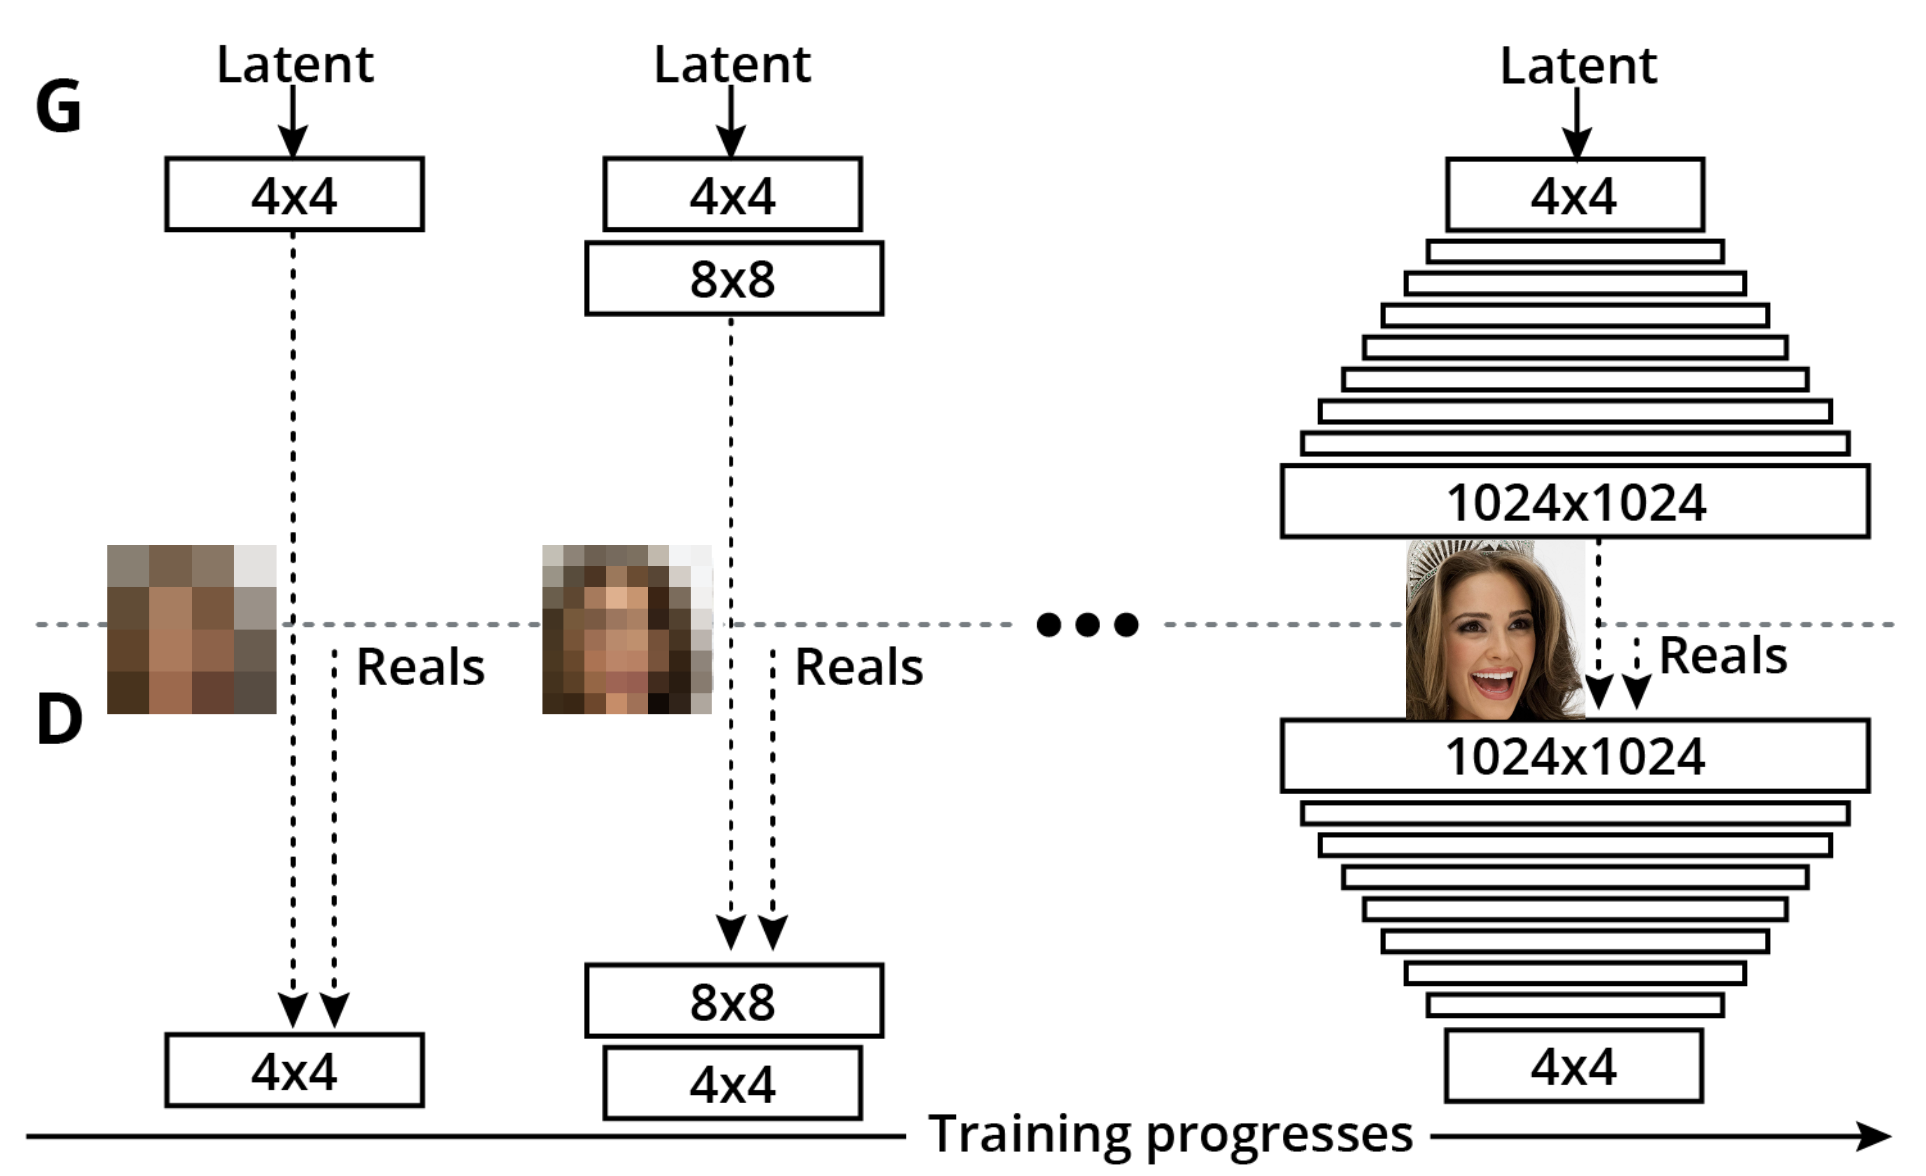
\includegraphics[width=1\linewidth]{img//genAdvNet//modernGAN/progan2.png}

\subsection{Layer fading}
Each level, or depth, is training for a certain number of epochs (eg, 10
epochs). Then a new layer is added in the discriminator and the
generator and we start training with these additional layers. However,
when a new layer is added, it is fadded in smoothly, as described by the
following figure:

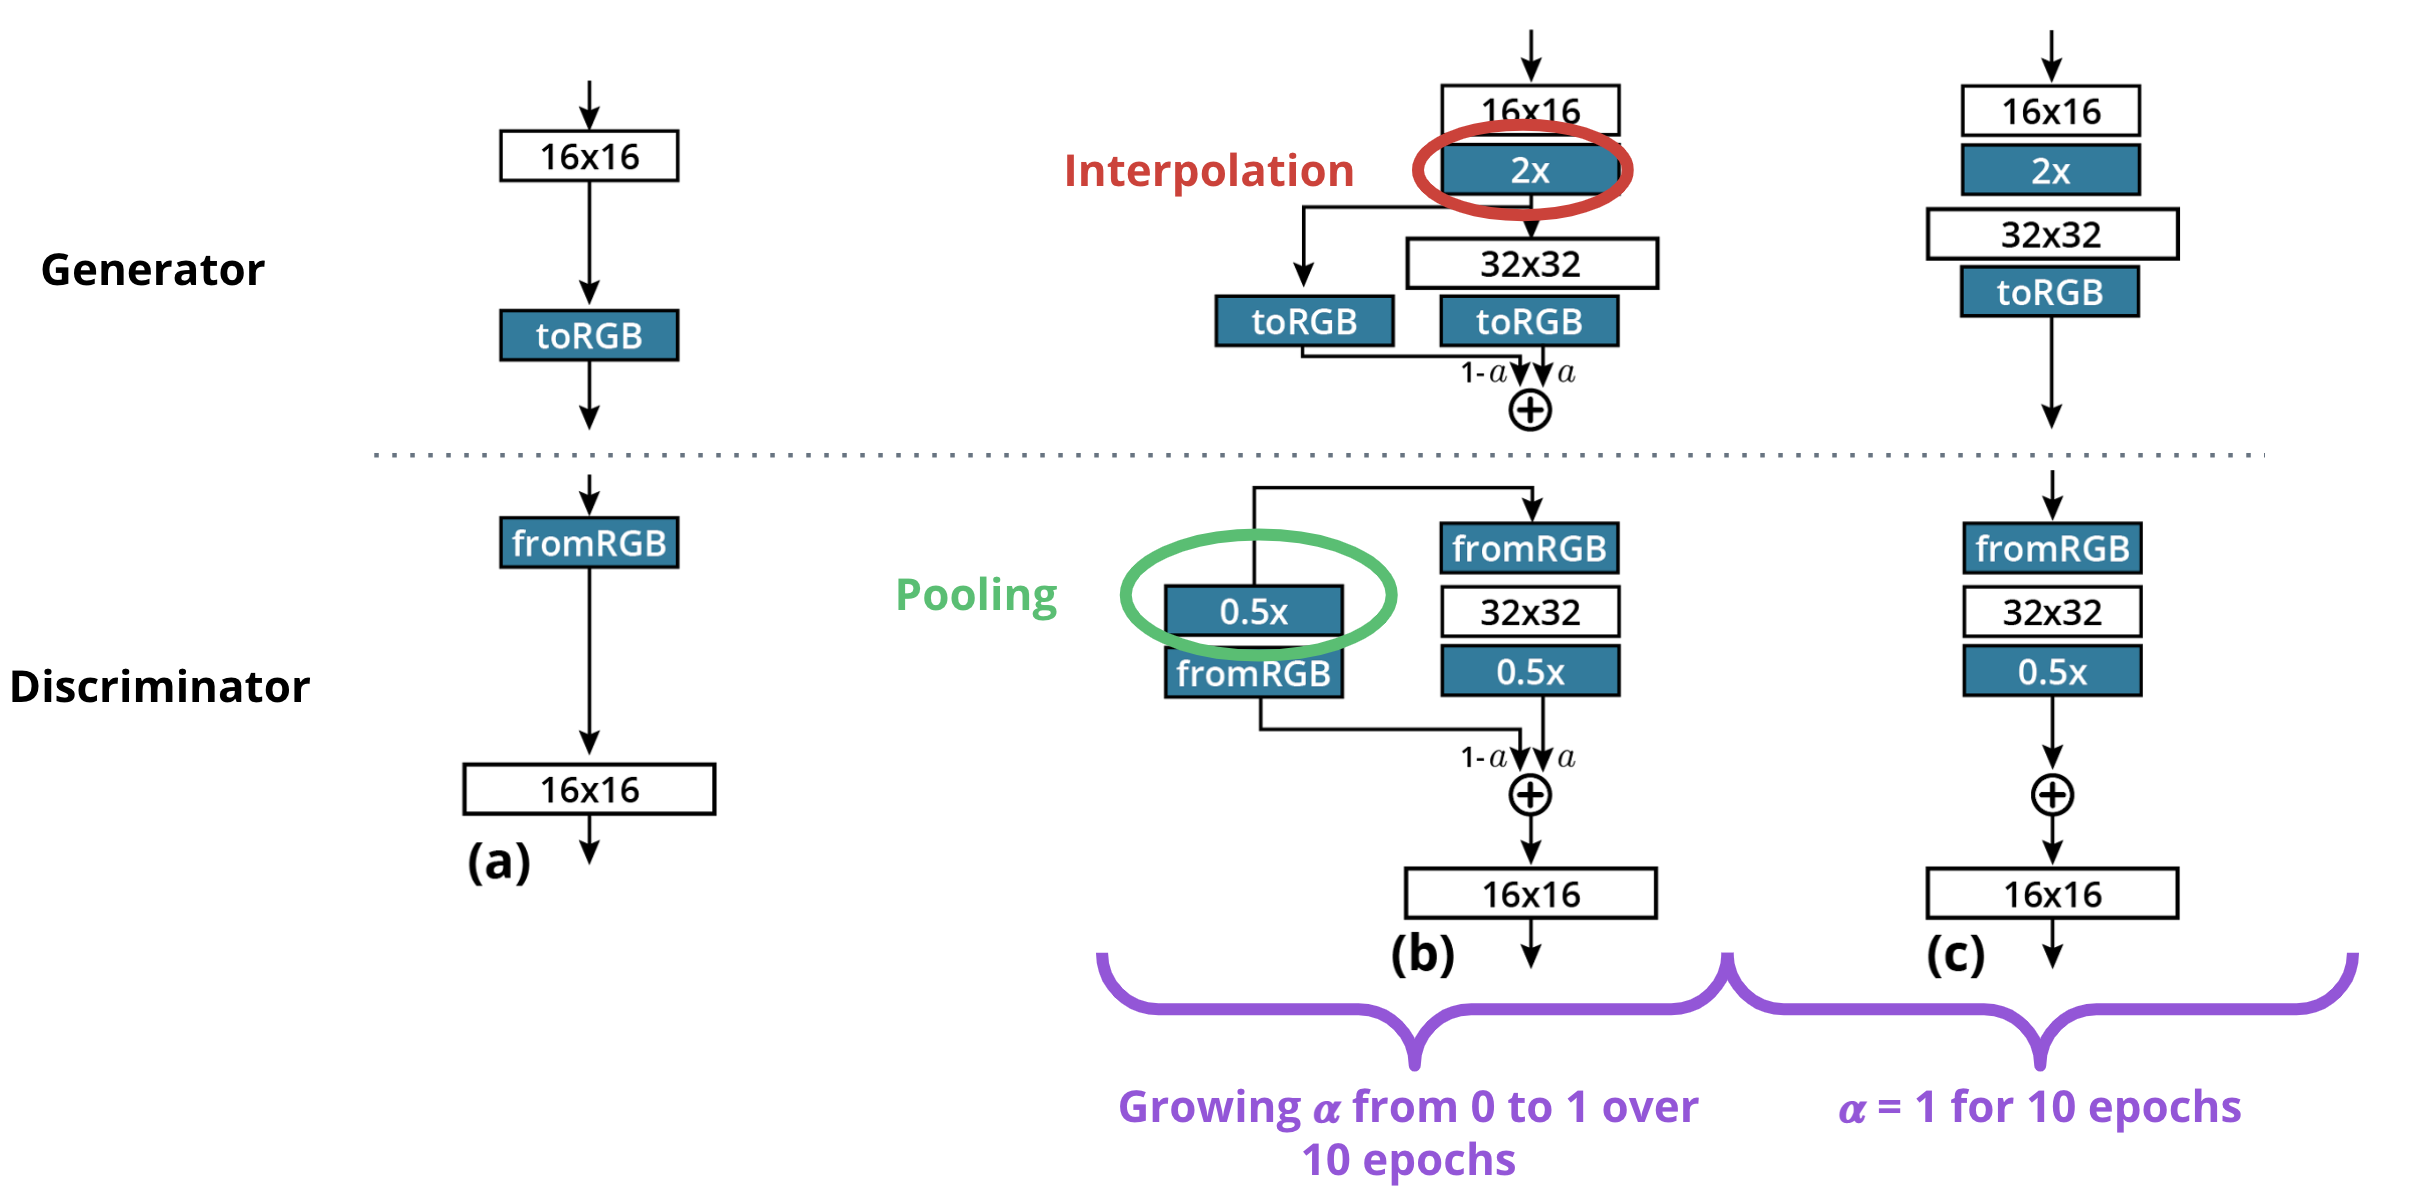
\includegraphics[width=1\linewidth]{img//genAdvNet//modernGAN/layer_fading2.png}

The \lstinline{toRGB} and
\lstinline{fromRGB} layers are the layers projecting the
feature vector to the RGB space (HxWx3) and the layer doing the
opposite, respectively. \newline

Let's look at the example: 
\begin{enumerate}[label=\textbf{(\alph*)}]
    \item the network is currrently training at 16x16 resolution, meaning that the generated images are 16x16x3
    \item we are adding two new layers to train at 32x32 resolution. However, we are fading the new layers by doing the following:
    \begin{itemize}
        \item for the generator, we take the output of the 16x16 layer and use nearest neighbor image resize to double its resolution to 32x32. The same output will also be fed to the 32x32 layer. Then we calculate the output of the network by doing a weighted sum of \((1- \alpha)\) the upsampled 16x16 image and \(\alpha\) the 32x32 layer output.
        \item for the discriminator, we do something similar but to reduce the resolution, we use an average pooling layer
        \item the network trains for N epochs at each resolution. During the first \(N/2\) epochs, we start with \(/alpha = 0\) and increase alpha linearly to \(/alpha = 1\). Then we train for the remaining \(N/2\) epochs with \(/alpha = 1\).
    \end{itemize}
    \item the network is now training at 32x32 resolution
\end{enumerate}

\subsubsection{Exercerise}
In this exercise, you will implement the Generator of the ProGan model. To make your life easier, I already implemented two torch modules: \lstinline{GeneratorFirstBlock} and \lstinline{GeneratorBlock}. 
\begin{itemize}
    \item The \lstinline{GeneratorFirstBlock} module takes the the latent vector as input and outputs a multi-dimensional feature maps
    \item the \lstinline{GeneratorBlock} module correspond to each layer added when increasing the resolution
\end{itemize}

\textbf{Notes:} In the paper, the authors are using a new type of normalization, called PixelNormalization. I encourage you to read the paper but for the sake of simplicity, I did not add any normalization here.

\begin{lstlisting}[language=Python]
import numpy as np
import torch
import torch.nn as nn
\end{lstlisting}

\begin{lstlisting}[language=Python]
class GeneratorFirstBlock(nn.Module):
    """
    This block follows the ProGan paper implementation.
    Takes the latent vector and creates feature maps.
    """
    def __init__(self, latent_dim: int):
        super(GeneratorFirstBlock, self).__init__()
        # initial block 
        self.conv0 = nn.ConvTranspose2d(latent_dim, 512, kernel_size=4)
        self.conv1 = nn.Conv2d(512, 512, kernel_size=3, padding=1)
        self.activation = nn.LeakyReLU(0.2)

    def forward(self, x: torch.Tensor):
        # x is a (batch_size, latent_dim) latent vector, we need to turn it into a feature map
        x = torch.unsqueeze(torch.unsqueeze(x, -1), -1)
        x = self.conv0(x)
        x = self.activation(x)
        
        x = self.conv1(x)
        x = self.activation(x)
        return x
\end{lstlisting}

\begin{lstlisting}[language=Python]
class GeneratorBlock(nn.Module):
    """
    This block follows the ProGan paper implementation.
    """
    def __init__(self, in_channels: int, out_channels: int):
        super(GeneratorBlock, self).__init__()

        self.conv1 = nn.Conv2d(in_channels, out_channels, 3, padding=1)
        self.conv2 = nn.Conv2d(out_channels, out_channels, 3, padding=1)
        self.activation = nn.LeakyReLU(0.2)

    def forward(self, x: torch.Tensor):
        x = interpolate(x, scale_factor=2)
        x = self.conv1(x)
        x = self.activation(x)

        x = self.conv2(x)
        x = self.activation(x)
        return x
\end{lstlisting}

Using the above two blocks, you can implement the Generator module. The end resolution that we want to reach is 512x512 and we will start at a 4x4 resolution.

\subsubsection{init}
The \lstinline{__init__} method should contain enough blocks to work at full resolution. We are only instantiating the generator once! So you will need to: 
\begin{itemize}
    \item create one GeneratorFirstBlock module
    \item create enough GeneratorBlocks modules such that the final resolution is 512x512
    \item create one \lstinline{toRGB} layer per resolution.
\end{itemize}

The number of filters in each layer is controlled by the \lstinline{num_filters} function below.

\subsubsection{forward}
The forward method does the following: 
\begin{itemize}
    \item takes the latent vector, the current resolution and \lstinline{alpha} as input.
    \item run the latent vector through the different blocks and perform \lstinline{alpha} fading
\end{itemize}

In the original paper, the number of filters of convolution layers increases with depth. The\lstinline{num_filters} function below will help you programmatically increase the number of filters based on the stage (or depth) of the generator. A depth of 1 correspond to 4x4 resolution, a depth of 2 to an 8x8 resolution etc.

\begin{itemize}
    \item you can the torch \lstinline{interpolate} function to double the resolution of an image
    \item you can use the \lstinline{np.log2} function to map the resolution of the input image to a ``depth'' (or stage) level. For example, \lstinline{np.log2(512) = 9} and \lstinline{np.log2(4)} = 2.
    \item when training at 4x4 resolution, you should not perform \(\alpha-\)fading.
\end{itemize}

\begin{lstlisting}[language=Python]
import tests

from torch.nn.functional import interpolate
\end{lstlisting}

\begin{lstlisting}[language=Python]
def num_filters(stage: int, 
                fmap_base: int = 8192,
                fmap_decay: float = 1.0,
                fmap_max: int = 512): 
    """
    A small helper function to computer the number of filters for conv layers based on the depth.
    From the original repo https://github.com/tkarras/progressive_growing_of_gans/blob/master/networks.py#L252
    """
    return min(int(fmap_base / (2.0 ** (stage * fmap_decay))), fmap_max)
\end{lstlisting}

\begin{lstlisting}[language=Python]
class Generator(nn.Module):
    """
    Generator: takes a latent vector as input and output an image.
    args:
    - max_resolution: max image resolution
    - latent_dim: dimension of the input latent vector
    """
    def __init__(self, max_resolution: int, latent_dim: int):
        super(Generator, self).__init__()

        # following the original implementation
        resolution_log2 = int(np.log2(max_resolution))

        # layers blocks
        self.blocks = [GeneratorFirstBlock(latent_dim)]
        for res in range(1, resolution_log2 - 1):
            self.blocks.append(GeneratorBlock(num_filters(res), num_filters(res+1)))
        self.blocks = nn.ModuleList(self.blocks)

        # to rgb blocks
        self.to_rgb = [nn.Conv2d(num_filters(res), 3, kernel_size=1) for res in range(1, resolution_log2)]
        self.to_rgb = nn.ModuleList(self.to_rgb)

    def forward(self, x: torch.Tensor, current_res: int, alpha: float = 1.0):
        resolution_log2 = int(np.log2(current_res))

        # to rgb operation
        if current_res == 4:
            x = self.blocks[0](x)
            images_out = self.to_rgb[0](x)
        else:
            # blocks
            for block in self.blocks[:resolution_log2-2]:
                x = block(x)

            previous_img = self.to_rgb[resolution_log2-3](x)
            previous_img_scaled = interpolate(previous_img, scale_factor=2)

            x = self.blocks[resolution_log2-2](x)
            new_img = self.to_rgb[resolution_log2-2](x)
            images_out = new_img * alpha + (1 - alpha) * previous_img_scaled
        return images_out
\end{lstlisting}

\begin{lstlisting}[language=Python]
generator = Generator(max_resolution=512, latent_dim=128)
\end{lstlisting}

\begin{lstlisting}[language=Python]
tests.check_progan_generator(generator)
\end{lstlisting}

\begin{lstlisting}[language=Python]
\end{lstlisting}


\section{Exercise 2: Solution}
\href{https://www.youtube.com/watch?v=-BK4Y_PIAag}{Youtube}

\section{StyleGAN: Introduction}
\href{https://www.youtube.com/watch?v=OI3t0u5DINc&t=2s}{Youtube} \newline

Deep learning is a somewhat recent field and many consider the 2012 AlexNet paper as the starting point of the deep learning revolution. The progress in creating realistic generated images is most exemplified by the StyleGAN paper in 2019 as it was the first architecture to produce very high-quality samples.

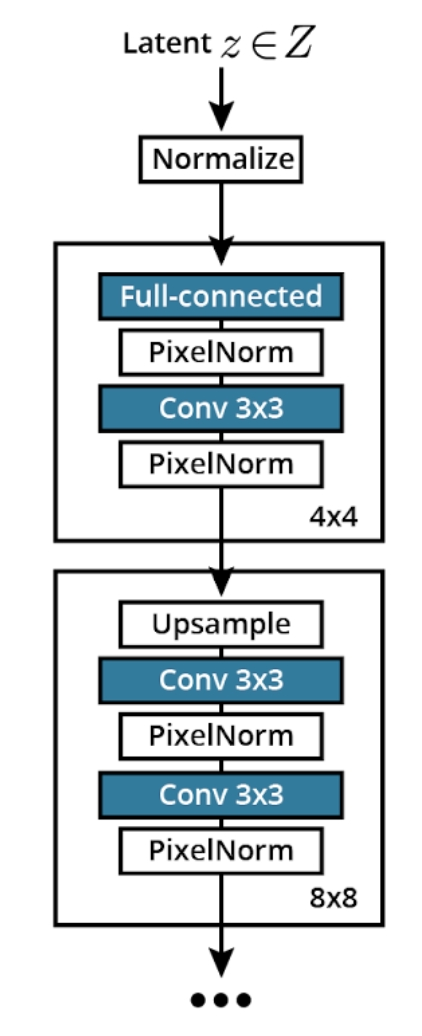
\includegraphics[width=0.25\linewidth]{img//genAdvNet//modernGAN/screen-shot-2022-06-30-at-4.12.15-pm.jpeg}
\captionof{figure}{Traditional generator}


\subsection{The Traditional Generator}
For a traditional generator:

\begin{enumerate}
    \item We input a latent vector z.
    \item Run it through a bunch of fully connected, convolution and normalization layers.
    \item Get a generated RGB image.
\end{enumerate}

\subsection{The StyleGAN Generator}
For the StyleGAN generator :

\begin{enumerate}
    \item There is a new network, only made of fully connected layer, \textbf{the mapping network,} and it is taking the latent vector and outputs a new latent vector w.
    \item Add noise at multiple places in the network, always after the convolution layers.
    \item StyleGAN uses a new type of normalization layer, the \textbf{adaptive instance normalization layer}, or \textbf{AdaIn}.
\end{enumerate}
Next, we will dissect each one of these new components and understand how they were leveraged to create such high quality images.

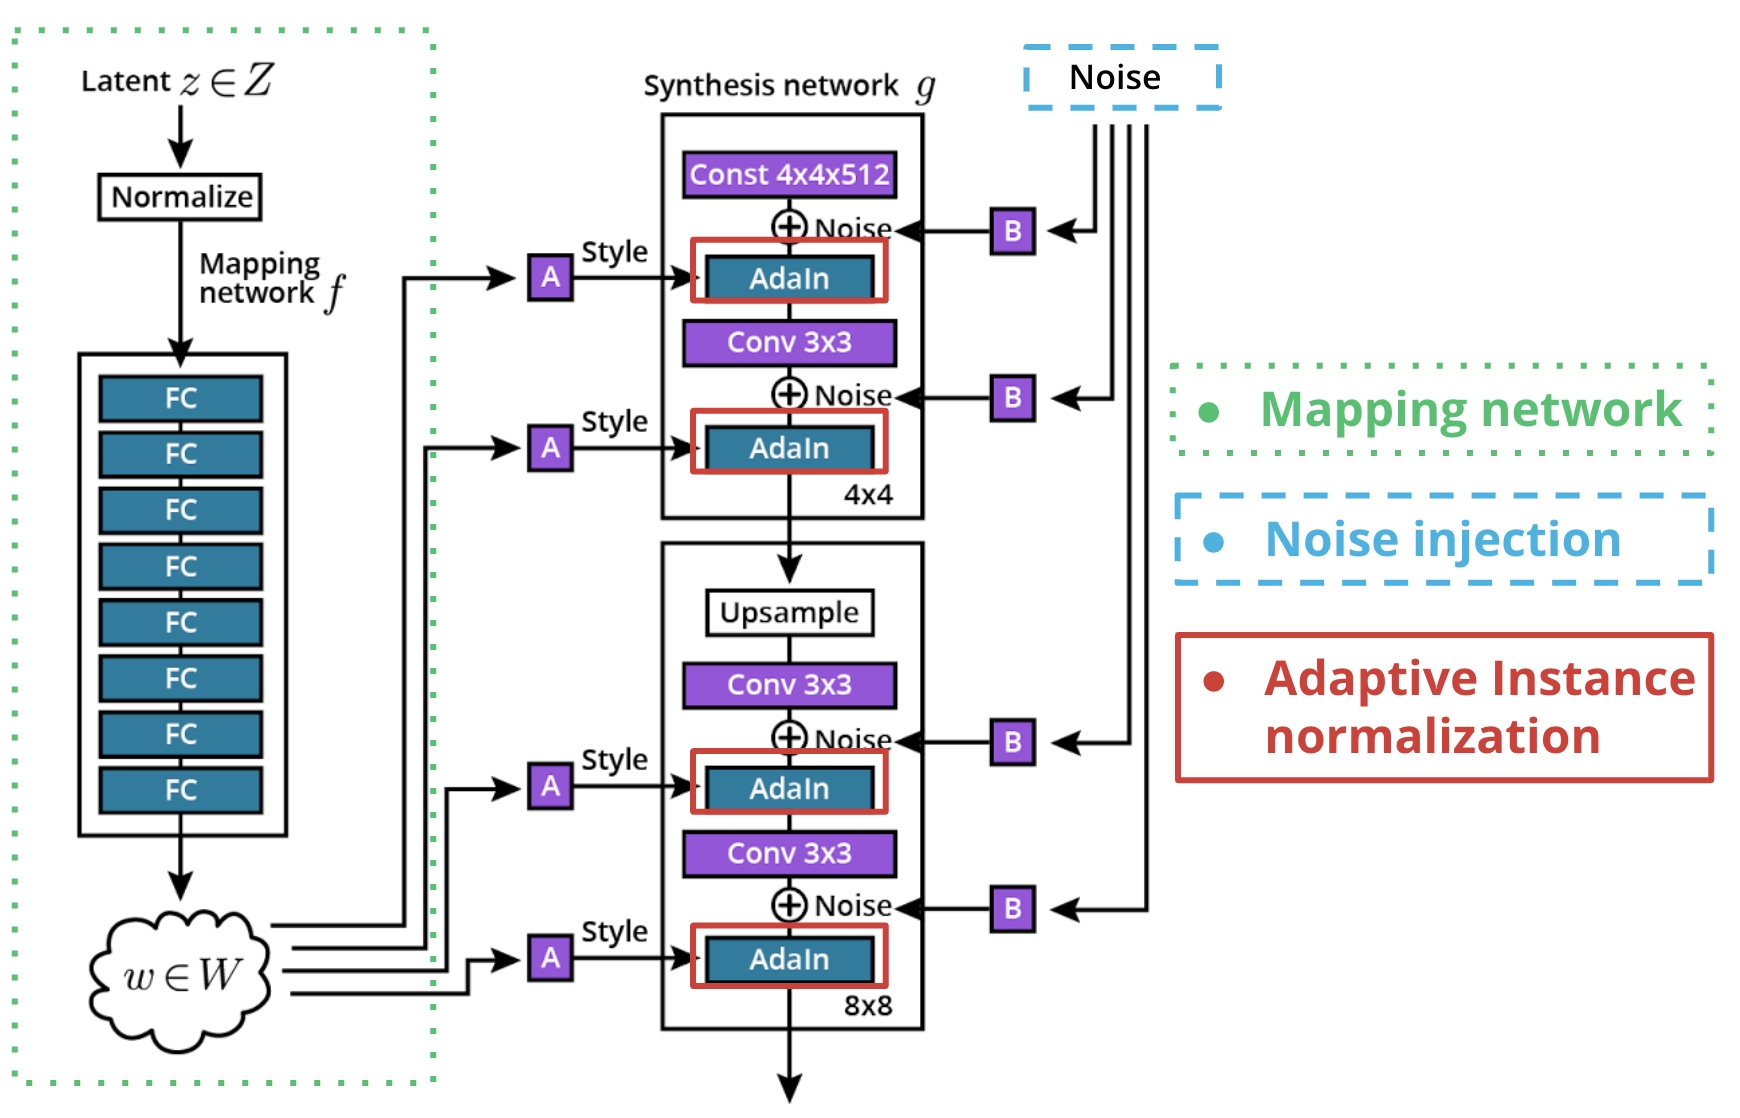
\includegraphics[width=1\linewidth]{img//genAdvNet//modernGAN/screen-shot-2022-06-30-at-4.13.35-pm.jpeg}
\captionof{figure}{StyleGAN architecture}


\subsection{Additional Resources}
The StyleGAN paper, \href{https://arxiv.org/pdf/1812.04948.pdf}{\textbf{A Style-Based Generator Architecture for Generative Adversarial Networks}} [1], is worth reading to explore the full details of the architecture. The images shown here are from the StyleGAN paper referenced.

\subsection{Citations}
Following is the full citation for the paper referenced on this page: \newline

\textbf{[1]} T. Karras, S. Laine, T. Aila, "\textit{A Style-Based Generator Architecture for Generative Adversarial Networks}", NVIDIA [Online], Available: \href{https://arxiv.org/pdf/1812.04948.pdf}{\textbf{https://arxiv.org/pdf/1812.04948.pdf}} . [Accessed June 28, 2022].

\section{StyleGAN Components 1}
\href{https://www.youtube.com/watch?v=FgWMN-FMdjU}{Youtube}

\subsection{Controllable Generation}
\textbf{Conditional Generation} indicates that the training set must be labeled and conditioning is limited to examples from the training set. \newline

\textbf{Conditional Generation} – each image is conditioned with a label (e.g. MNIST dataset).
For example, fake 11s can not be generated with a conditional GAN trained on the MNIST dataset because the data set only includes digits in the range of 0 to 9. \newline

\href{https://arxiv.org/pdf/1411.1784.pdf}{\textbf{Conditional Generative Adversarial Nets}} [1] introduced the \textbf{conditional GAN}. An example of conditional implementation in PyTorch can be viewed in the \href{https://github.com/eriklindernoren/PyTorch-GAN/blob/36d3c77e5ff20ebe0aeefd322326a134a279b93e/implementations/cgan/cgan.py}{\textbf{PyTorch-GAN CGAN implementation on GitHub}}. Conditional GANs have an extra input from the discriminator and generator networks. \newline

For \textbf{controllable generation,} instead of inputting a label to condition the output, the latent vector z is modified to control the aspect of the output. This makes the assumption that the components of z each control a different aspect of the output image. 

\begin{itemize}
    \item \textbf{Controllable Generation} – does not require labels.
\end{itemize}

\subsection{The Mapping Network}
The \textbf{mapping network} is a new component of the StyleGAN generator. A mapping network:

\begin{itemize}
    \item Takes the latent vector z as input
    \item Outputs a new latent vector w
    \item Helps to disentangle the latent vector z for controllable generation = decorrelate the different features
\end{itemize}

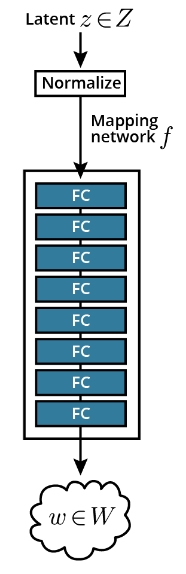
\includegraphics[width=0.25\linewidth]{img//genAdvNet//modernGAN/screen-shot-2022-06-30-at-4.46.39-pm.jpeg}
\captionof{figure}{StyleGAN: mapping network}

\subsection{The Entanglement Problem}
When modifying some components, we impact more than one feature. Some features are correlated or entangled. This is the \textbf{entanglement problem}. \newline

For example in trying to generate faces, features could include:
\begin{itemize}
    \item Haircut
    \item Eye color
    \item Glasses
    \item Age
\end{itemize}

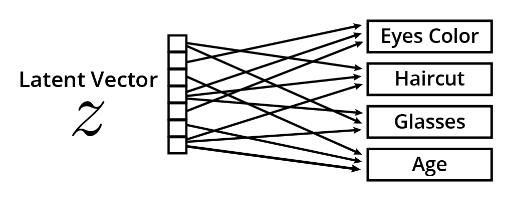
\includegraphics[width=0.5\linewidth]{img//genAdvNet//modernGAN/screen-shot-2022-06-30-at-4.46.56-pm.jpeg}
\captionof{figure}{The entanglement problem}

If the features are entangled, putting glasses on a person could also make them older. \newline

Mapping network to the rescue! By mapping the vector z to another vector w, the generator gets the capacity to disentangle features.
\subsection{Noise Injection}
Another new component of StyleGAN is the injection of noise at different locations in the generator. This \textbf{noise injection} will:

\begin{itemize}
    \item Help with \textbf{stochastic variation}, e.g. the position of freckles on a face. Injecting noise in the network will help create more diverse features.
    \item Happen at different locations in the network and impacts the variability of the images at different levels.
\end{itemize}
A \textbf{learned scaling factor} is applied to the noise input before being added to the output of a given layer. \newline

To add noise:
\begin{enumerate}
    \item A random feature map is sampled from a gaussian distribution
    \item The map is multiplied by a learned scaling factor
    \item This noise is applied to the output of the convolutional layers
\end{enumerate}

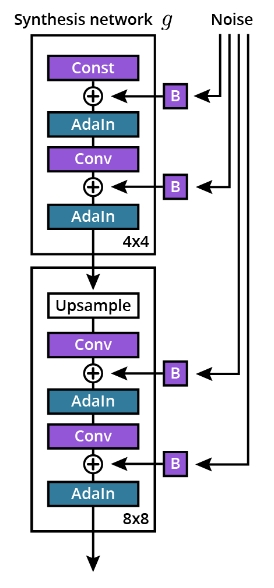
\includegraphics[width=0.5\linewidth]{img//genAdvNet//modernGAN/screen-shot-2022-06-30-at-4.47.08-pm.jpeg}
\captionof{figure}{Noise injection}

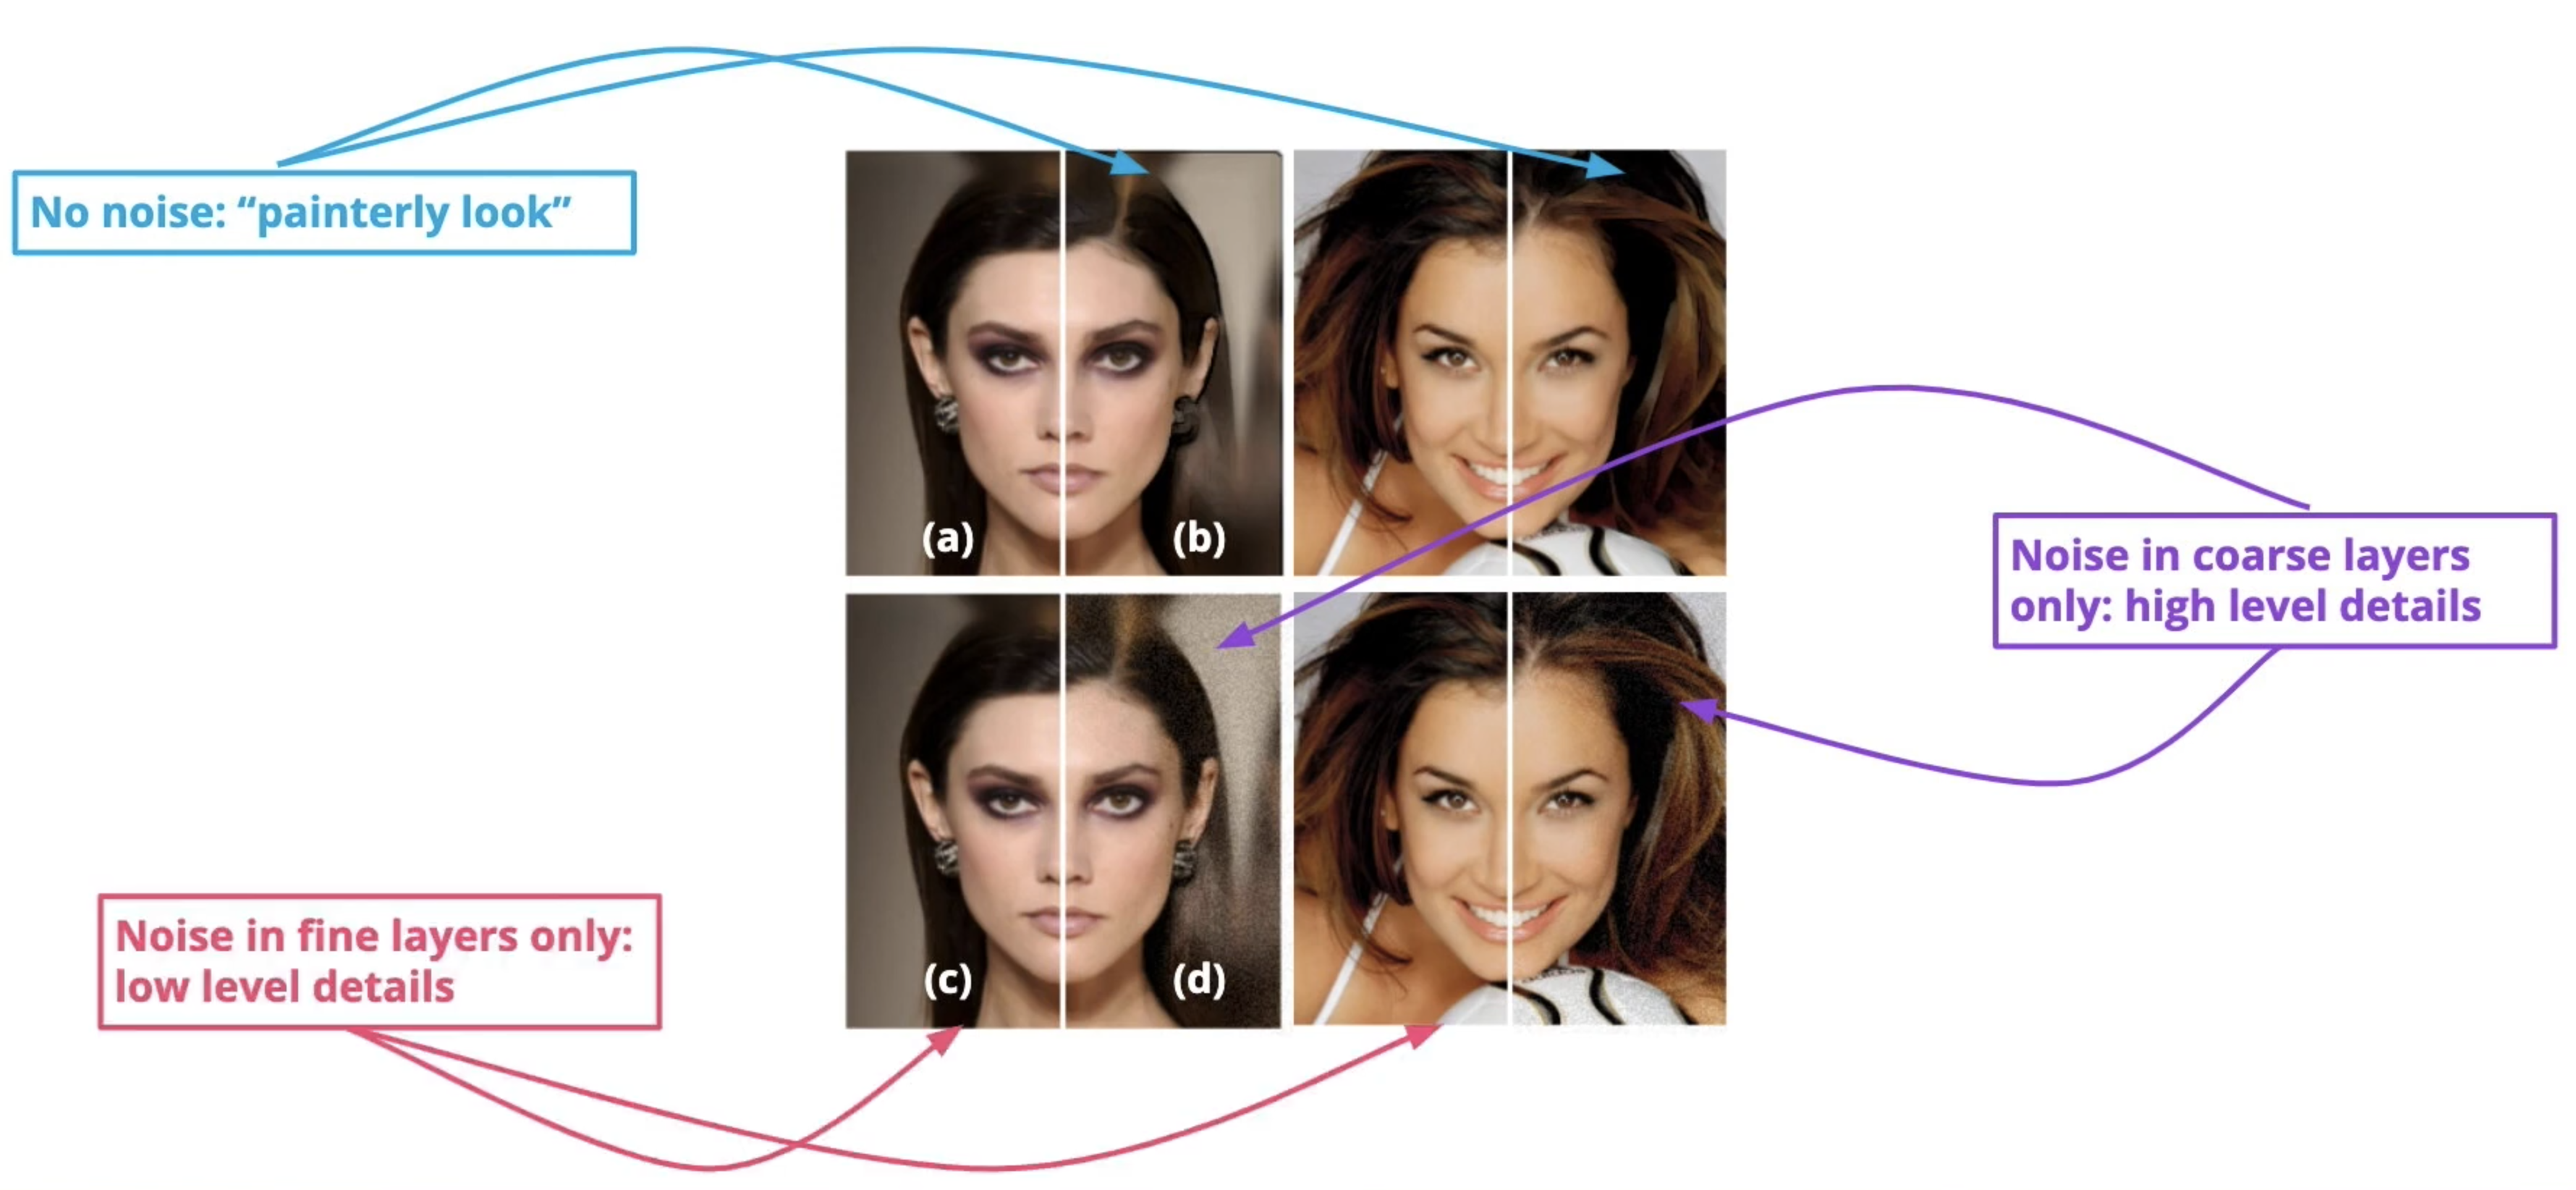
\includegraphics[width=1\linewidth]{img//genAdvNet//modernGAN/noiseVSnoNoise.png}
\captionof{figure}{Comparison between noise vs no noise}

\subsection{Citations}
Following are the full citations for the papers referenced on this page: \newline

\textbf{[1]} M. Mirza, S, Osindero, "\textit{Conditional Generative Adversarial Nets}", Departement d’informatique et de recherche operationnelle Universite de Montreal, Flickr / Yahoo Inc. [Online], Available: \href{https://arxiv.org/pdf/1411.1784.pdf}{\textbf{https://arxiv.org/pdf/1411.1784.pdf}}. [Accessed June 28, 2022].

\section{SyleGAN Components 2}
\href{https://www.youtube.com/watch?v=Cs467j73Ml0&t=3s}{Youtube} \newline

All \textbf{Normalization Layers} calculate the mean and the variance of a certain subset and normalize the input. \newline

Remember, for \textbf{Batch Normalization}, we:

\begin{enumerate}
    \item Calculate the mean and variance of the batch and spatial dimensions
    \item For each channel of the inputs, there are different values of means and variance
\end{enumerate}

\subsection{Instance Normalization Layer}
The \textbf{Instance Normalization Layer} – only normalizes over the spatial dimensions and each input has a number of channels times the batch size values of means and variance.

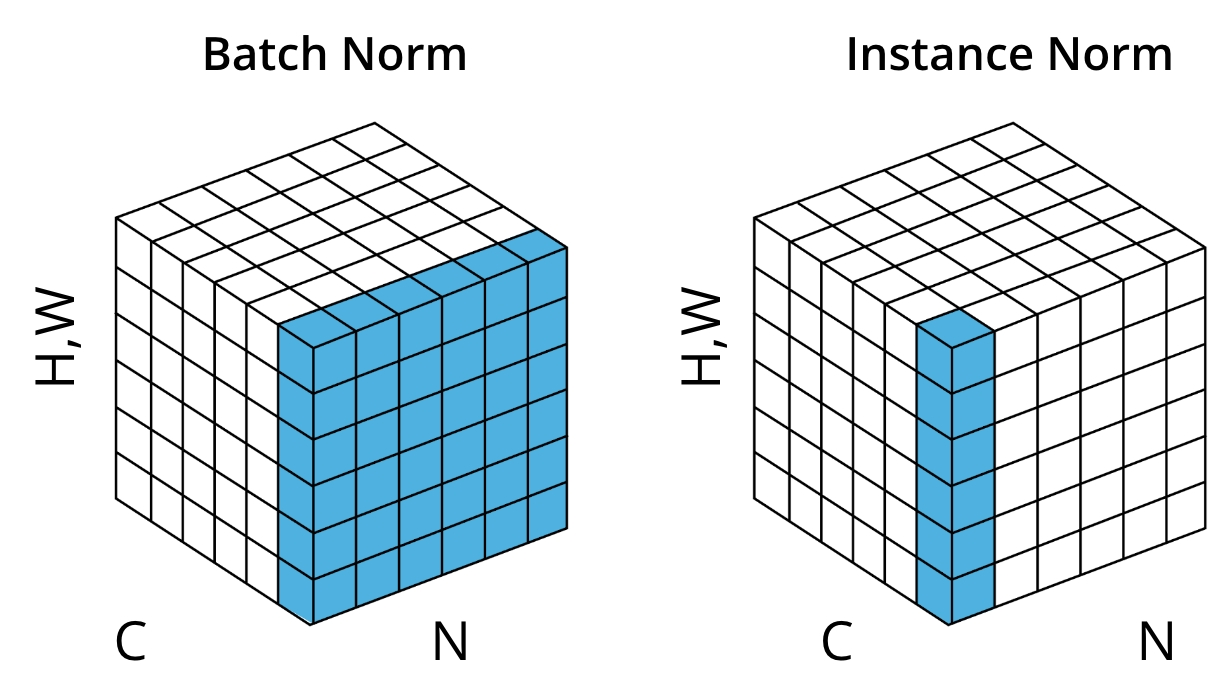
\includegraphics[width=0.5\linewidth]{img//genAdvNet//modernGAN/screen-shot-2022-06-30-at-6.23.29-pm.jpeg}
\captionof{figure}{Image adapted from: \href{https://arxiv.org/pdf/1803.08494v3.pdf}{\textbf{https://arxiv.org/pdf/1803.08494v3.pdf}}}

\subsection{Adaptive Instance Normalization Layer}
The \textbf{Adaptive Instance Normalization Layer (Adaln):}

\begin{enumerate}
    \item Takes the latent vector, \(w\), as input and using a fully connected layer, projects that vector into two vectors of style, \(y_s\) and \(y_b\).
    \item The output of the previous layer goes through an Instance Normalization Layer.
    \item Use the styles \(y_s\) and \(y_b\) to scale and bias the output of the Instance Normalization Layer.
    \item Allows one to project the latent vector \(w\) into the styles and inject the styles into the generator.
\end{enumerate}
\textbf{Style Mixing} injects a different vector \(w\) at different places in the network and provides a regularization effect. This prevents the network from assuming that adjacent styles are correlated.

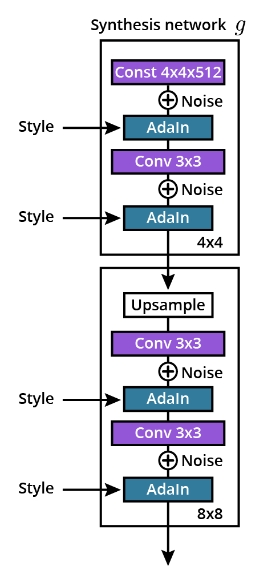
\includegraphics[width=0.5\linewidth]{img//genAdvNet//modernGAN/screen-shot-2022-06-30-at-6.26.28-pm.jpeg}
\captionof{figure}{Adaptive Instance Normalization (AdaIn) layer}


\subsection{Style Transfer}
In practice, Adaln layers allow for the creation of a new image (c) by taking a first image (a) and modifying it in the style of a second image (b). A popular example is taking the image of the Mona Lisa (a) and the style of a Picasso painting (b) and creating a new Mona Lisa in Picasso style image (c). This image can be seen \href{https://www.deviantart.com/dr-koesters/art/Neural-Style-Transfer-Mona-Lisa-by-Picasso-733533838}{\textbf{here}} and this process is known as \textbf{style transfer}. \newline

The initial process of style transfer was time consuming; however, check out the paper, \href{https://arxiv.org/pdf/1703.06868.pdf}{\textbf{\textit{Arbitrary Style Transfer in Real-time with Adaptive Instance Normalization}}}, which details a use case for how Adaln layers may be implemented to create fast style transfers based on arbitrary styles.

\subsection{Entanglement}
In your own words, explain the problem of feature entanglement and how StyleGAN tries to solve it. \newline

Things to think about: The StyleGAN paper (section 4) goes into depth about disentanglement. Definitely a recommended read!

\subsection{Quiz Question}
Match each element of the StyleGAN model with its purpose

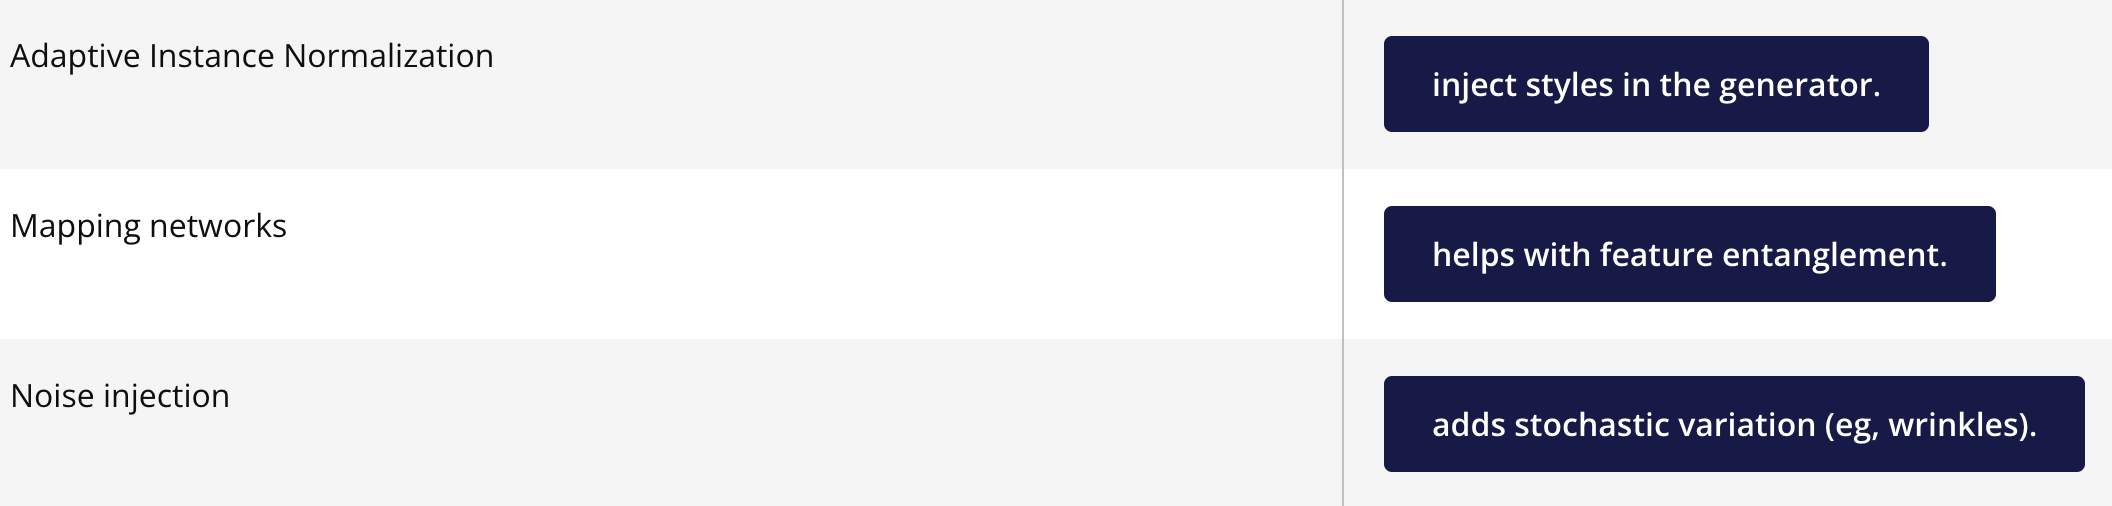
\includegraphics[width=1\linewidth]{img//genAdvNet//modernGAN/quiz_styleGAN.png}

\subsection{Citations}
Following are the full citations for the papers referenced on this page: \newline

\textbf{[1]} X. Huang, S. Belongie, "\textit{Arbitrary Style Transfer in Real-time with Adaptive Instance Normalization}", Department of Computer Science \& Cornell Tech, Cornell University [Online], Available: \href{https://arxiv.org/pdf/1703.06868.pdf}{\textbf{https://arxiv.org/pdf/1703.06868.pdf}}. [Accessed June 30, 2022].
\section{Exercise 3: StyleGan}

Look at this: \url{https://thispersondoesnotexist.com/} ! Would you
believe this picture is not real??? Well it is not! Feel free to refresh
the page to look at more examples. This picture has been generated by
\href{https://arxiv.org/pdf/1812.04948.pdf}{StyleGan}, a groundbreaking
architecture in the world of GANs! \newline

The StyleGan uses a lot of tricks that we have seen in the course (eg,
progressive growing) but also relies on a novel approach to controlled
generation. The figure below describes the architecture of the network: \newline

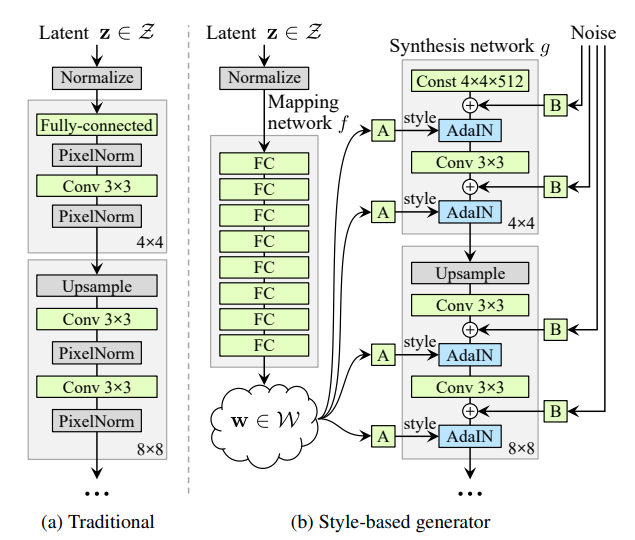
\includegraphics[width=1\linewidth]{img//genAdvNet//modernGAN/stylegan.png}

Wow! We have a completely new network in our GAN. This network is called
the \textbf{noise mapping} network. The architecture of this network is
fairly simple, it only consists of 8 fully connected layers. The authors
argue that mapping the latent vector \(z\) to a new latent vector \(w\)
facilitates \textbf{disentanglement}. \newline

We talked about disentanglement in the course: when modifying the latent
vector \(z\) to control the aspect of the generated image, we often face
entangled features. For example, longer hair can be correlated with a
more feminine face. Using the mapping vector in StyleGan facilities the
decorrelation of such features. \newline

What happens next? The generated \(w\) latent vector is injected into a
``classic'' generator network. However, this network has two components
you are not yet familiar with, as seen in the figure above. Indeed,
after each convolution layer, we see that the authors are adding
\textbf{noise}. Moreover, the convolution output with added noise is
then fed into a \textbf{adaptive instance normalization layer or AdaIN}.  \newline

In this notebook, you will implement a \textbf{noise injection layer}
and the \textbf{AdaIn layer}.

\subsection{Noise injection}
The noise injection helps with something that the authors call
\textbf{stochastic variation}. They argue that many aspects of a human
face are stochastic, such as hair curls or freckles. By adding random
noise at different levels in the generator, they can create more
variability without changing the overall image. For example in the image
below, we can see how different noise vectors impacts the placement of
the hair.

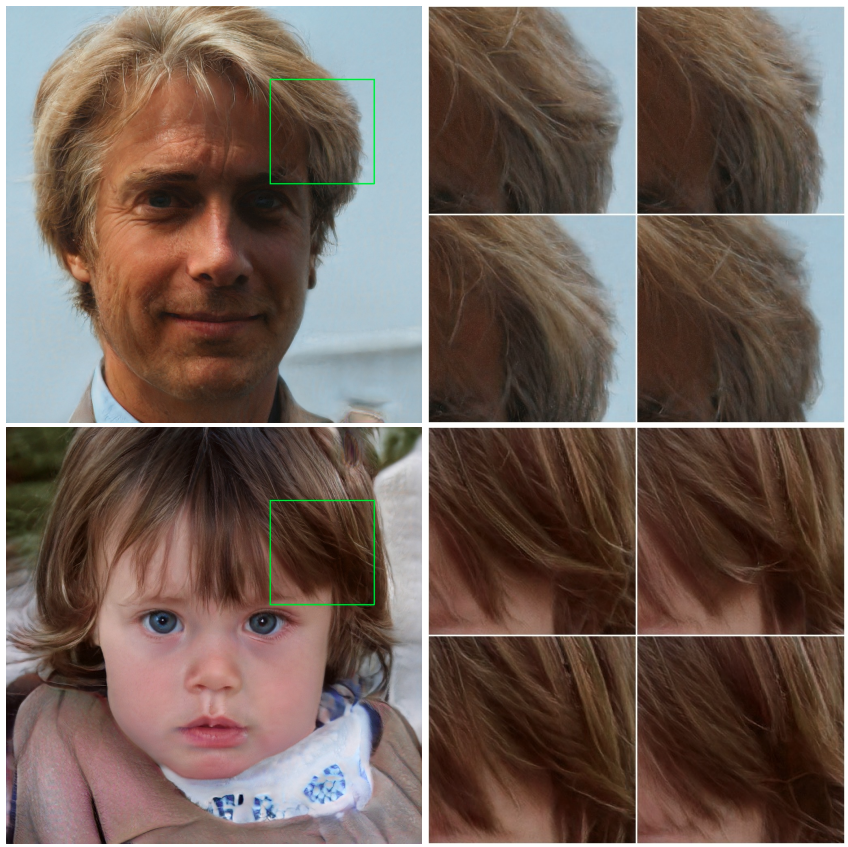
\includegraphics[width=0.5\linewidth]{img//genAdvNet//modernGAN/stochastic_variation.png}

After each convolution layer in the generator, the authors added a noise
injection layer. A random gaussian noise is added to the output and
scaled by a learned factor. Let's look at an example together: 
\begin{itemize}
    \item let's say that the output shape of the convolution layer is \lstinline{(1, 256, 32, 32)} where 256 is the number of channels and 32x32 the spatial dimensions.
    \item we create a random noise matrix of dimensions \lstinline{(1, 1, 32, 32)}
    \item we multiply the above random by a learned scaling factor vector of dimensions \lstinline{(1, 256, 1, 1)}. This learned scaling factor is initialized with zeros.
\end{itemize}

For the first exercise of this notebook, you will implement the
\lstinline{ApplyNoise} layer.

Click for tips

\begin{itemize}
\item You can read about custom pytorch modules implementation \href{https://pytorch.org/tutorials/beginner/examples_nn/two_layer_net_module.html}{here}.
\end{itemize}

\begin{lstlisting}[language=Python]
import torch
import torch.nn as nn

import tests
\end{lstlisting}

\begin{lstlisting}[language=Python]
class ApplyNoise(nn.Module):
    """
    Noise injection layer with learnable parameters.
    
    args:
    - channels: number of channels of the input
    """
    def __init__(self, channels: int):
        super(ApplyNoise, self).__init__()
        self.channels = channels
        self.weights = nn.Parameter(torch.zeros(1, channels, 1, 1))
    
    def forward(self, x: torch.Tensor) -> torch.Tensor:
        noise = torch.randn(1, 1, x.shape[2], x.shape[3])
        x = x + self.weights * noise
        return x
\end{lstlisting}

\begin{lstlisting}[language=Python]
apply_noise = ApplyNoise(512)
\end{lstlisting}

\begin{lstlisting}[language=Python]
tests.check_apply_noise(apply_noise)
\end{lstlisting}

\begin{lstlisting}
Congrats, you successfully implemented a noise injection layer!
\end{lstlisting}

\subsection{Adaptive instance normalization}
The Adaptive instance normalization (AdaIN) is a variation of the
\textbf{Instance Normalization layer}. In the course, we have discussed
about the importance of Batch Normalizations layers. However, we also
have seen that in some cases (eg, when using gradient penalties), Batch
Normalization is not the preferred type of normalization layer. \newline

This figure from the \href{https://arxiv.org/pdf/1803.08494.pdf}{Group
Normalization} paper helps to understand the differences between the
normalization layers. In the figure below, \(H\) and \(W\) are the
spatial dimensions, \(C\) the channel dimension and \(N\) the batch
dimension.

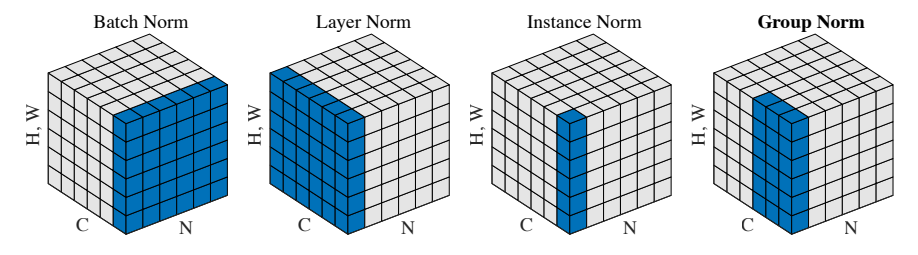
\includegraphics[width=1\linewidth]{img//genAdvNet//modernGAN/normalization_layers.png}

In\href{https://pytorch.org/docs/stable/generated/torch.nn.BatchNorm2d.html}{\textbf{Batch Normalization}}, we normalize pixels of the same channel, accross the batch and spatial dimensions. \newline

In \href{https://pytorch.org/docs/stable/generated/torch.nn.LayerNorm.html}{\textbf{Layer Normalization}}, we normalize pixels of the same batch index, accross the channel and spatial dimensions. \newline

In \href{https://pytorch.org/docs/stable/generated/torch.nn.InstanceNorm2d.html}{\textbf{Instance Normalization}}, we normalize pixels of the same batch index and channel, accross the spatial dimensions only. \newline

In \href{https://pytorch.org/docs/stable/generated/torch.nn.GroupNorm.html}{\textbf{Group Normalization}}, we group pixels of the batch index together. \newline

The AdaIN layer is an extension of the Instance Normalization layer. It
takes as input both the output of the previous convolution layer and the
latent vector \(w\). Then it performs the following: 
\begin{itemize}
    \item map the latent vector \(w\) to styles vector \((y_{s}, y_{b})\) through learned affine transformations (fully connected layers).
    \item calculate the output of the layer using the following equation: \(y_{s} * In(x) + y_{b}\) where \(In(x)\) is the input \(x\) fed through an instance normalization layer.
\end{itemize}

For the second exercise in this notebook, you will implement the AdaIN
layer.

\textbf{Tip:}

\begin{itemize}
\item You can use the torch Instance Normalization module for an easier implementation.
\end{itemize}

\begin{lstlisting}[language=Python]
class AdaIN(nn.Module):
    """
    Adaptive Instance Normalization layer
    
    args:
    - channels: number of channels of the input
    - w_dim: dimension of the latent vector w
    
    inputs:
    - x: float32 tensor of dim [N, C, H, W]
    - w: float32 tensor of dim [N, W_DIM]
    """
    def __init__(self, channels: int, w_dim: int):
        super(AdaIN, self).__init__()
        self.channels = channels
        self.w_dim = w_dim
        self.instance_norm  = nn.InstanceNorm2d(channels)
        self.linear_s = nn.Linear(w_dim, channels)
        self.linear_b = nn.Linear(w_dim, channels)
        
    def forward(self, x: torch.Tensor, w: torch.Tensor) -> torch.Tensor:
        x = self.instance_norm(x)       
        ys = self.linear_s(w)[..., None, None]
        yb = self.linear_b(w)[..., None, None]
        return x * ys + yb
\end{lstlisting}

\begin{lstlisting}[language=Python]
adain = AdaIN(512, 128)
\end{lstlisting}

\begin{lstlisting}[language=Python]
tests.check_adain(adain)
\end{lstlisting}

\begin{lstlisting}
Congrats, you successfully implemented the AdaIN layer!
\end{lstlisting}

\section{Exercise 3: Solution}
\href{https://www.youtube.com/watch?v=6E98tNss7Y8}{Youtube}

\section{When to Use Modern GAN Techniques}
Youtube \newline

Starting with a simpler architecture is always an easy and fast way to get started on a new problem.
\begin{itemize}
    \item \textbf{DCGAN} is great starting point
    \item \textbf{ProGAN} or \textbf{StyleGAN} are practical when training on high resolution images
    \item \textbf{Wasserstein Loss} and \textbf{Gradient Penalties} experimentation is recommended when mode collapse or vanishing gradient are observed
\end{itemize}

\subsection{Additional Resources}
One of my favorite blog posts ever: \href{http://karpathy.github.io/2019/04/25/recipe/}{\textbf{A recipe for training neural networks(opens in a new tab)}}. A great read and most concepts are applicable to GANs.

\section{Lesson Review}
\href{https://www.youtube.com/watch?v=sX7084PStFk}{Youtube} \newline

We have completed this lesson on implementing \textbf{Modern GAN} modeling techniques and you have accomplished a lot. \newline

Over the course of this lesson you:
\begin{itemize}
    \item Used the Wasserstein Distance as a Loss Function for Training GANs
    \item Leveraged Gradient Penalties to Stabilize GAN Model Training
    \item Built a ProGAN Model
    \item Built Components of a StyleGAN Model
\end{itemize}
\textbf{Congratulations, work well done!}

\subsection{Citations}
Following are the full citations for the papers referenced on this page:

\begin{itemize}
    \item I. Goodfellow, J. Pouget-Abadie, M. Mirza, et al, "\textit{\textbf{Generative Adversarial Nets}}", Departement d’informatique et de recherche operationnelle Universite de Montreal [Online], Available: \href{https://arxiv.org/pdf/1406.2661.pdf}{\textbf{https://arxiv.org/pdf/1406.2661.pdf(opens in a new tab)}}. [Accessed June 28, 2022].
    \item X. Mao, Q. Li, H. Xie, R. Y.K. Lau, et al, "\textit{\textbf{Least Squares Generative Adversarial Networks}}", Department of Computer Science, City University of Hong Kong, Department of Mathematics and Information Technology, The Education University of Hong Kong, et al [Online], Available: \href{https://arxiv.org/pdf/1611.04076.pdf}{\textbf{https://arxiv.org/pdf/1611.04076.pdf(opens in a new tab)}}. [Accessed June 28, 2022].
    \item M. Arjovsky, S. Chintala, and L. Bottou, "\textit{\textbf{Wasserstein GAN}}", Courant Institute of Mathematical Sciences, Facebook AI Research [Online], Available: \href{https://arxiv.org/pdf/1701.07875.pdf}{\textbf{https://arxiv.org/pdf/1701.07875.pdf(opens in a new tab)}}. [Accessed June 28, 2022].
    \item I. T. Karras, T. Aila, S. Laine, J. Lehtinen, "\textit{\textbf{Progressive Growing GANs for Improved Quality, Stability, and Variation}}", NVIDIA, Aalto University [Online], Available: \href{https://arxiv.org/pdf/1710.10196.pdf}{\textbf{https://arxiv.org/pdf/1710.10196.pdf(opens in a new tab)}}. [Accessed June 28, 2022]
    \item Y. Wu, K. He, "\textit{\textbf{Group Normalization}}", Facebook AI Research (FAIR) [Online], Available: \href{https://arxiv.org/pdf/1803.08494.pdf}{\textbf{https://arxiv.org/pdf/1803.08494.pdf(opens in a new tab)}}. [Accessed June 28, 2022].
    \item T. Salimans, I. Goodfellow, W. Zaremba, et al, "\textit{\textbf{Improved Techniques for Training GANs}}", OpenAI [Online], Available: \href{https://arxiv.org/pdf/1606.03498.pdf}{\textbf{https://arxiv.org/pdf/1606.03498.pdf(opens in a new tab)}}. [Accessed June 28, 2022].
\end{itemize}

\section{Course Summary}
\href{https://www.youtube.com/watch?v=1R5JD_I3m0w}{Youtube} \newline

\subsection{Congratulations}
You have completed this course. We covered a number of topics and you implemented a broad variety of techniques, including:

\begin{itemize}
    \item Building and training a simple GAN model on the MNIST dataset
    \item Building a more complex DCGAN and implementing GAN evaluation metrics
    \item Using dataloaders and implementing functions to train a CycleGAN model
    \item Implementing gradient penalties to execute ProGAN and StyleGAN models
\end{itemize}
Congratulations again and we can't wait to see what innovative computer-generated images you create.
